\documentclass{espol-rte}

\usepackage[backend=biber,style=apa,sortcites=true,sorting=nyt]{biblatex}
\DeclareLanguageMapping{spanish}{spanish-apa}
\addbibresource{referencias_espol.bib}
\graphicspath{{../figures/}}
\usepackage{gensymb}

\renewcommand{\RTEtituloES}{Implementación y validación experimental de un sistema de retrofitting IoT para el estudio del MRUA en un entorno híbrido de aprendizaje}
\renewcommand{\RTEtituloEN}{Implementation and Experimental Validation of an IoT Retrofitting System for UARM Study in a Hybrid Learning Environment}
\renewcommand{\RTEautores}{%
  Walter Santiago Sosa Mej\'ia\textsuperscript{1}\,
  \href{https://orcid.org/0009-0003-6240-3462}{ORCID};
  Manuel Rogelio Nev\'arez Toledo\textsuperscript{1,*}\,
  \href{https://orcid.org/0000-0001-5628-3351}{ORCID}}
\renewcommand{\RTEafiliaciones}{%
  \textsuperscript{1}Pontificia Universidad Cat\'olica del Ecuador,
  Sede Esmeraldas, Esmeraldas, Ecuador\\
  wssosa@pucese.edu.ec; manuel.nevarez@pucese.edu.ec\\
  *Autor de correspondencia: manuel.nevarez@pucese.edu.ec}

\begin{document}
\makertetitle

\begin{resumenespol}
Se presenta el dise\~no, implementaci\'on y validaci\'on t\'ecnica de un prototipo de experimento remoto de cinem\'atica para el estudio del Movimiento Rectil\'ineo Uniformemente Acelerado (MRUA), desarrollado mediante una estrategia de \textit{retrofitting} con tecnolog\'ias de Internet de las Cosas (IoT) aplicadas sobre equipamiento preexistente de bajo costo. La arquitectura propuesta integra un microcontrolador ESP32 con procesamiento Edge computing, cuatro sensores infrarrojos de posici\'on, un broker MQTT en Raspberry Pi~4 y una interfaz web desarrollada en Next.js/React para control y visualizaci\'on en tiempo real. Con el objetivo de validar la equivalencia experimental entre la modalidad remota y la presencial, se ejecutaron 70 ensayos independientes (35 remotos y 35 presenciales) bajo condiciones controladas. Los resultados cuantitativos demuestran que las diferencias de medias entre modalidades son inferiores a 0{,}03~s en todos los puntos de medici\'on, con desviaciones est\'andar que difieren en menos de 0{,}02~s y aceleraciones experimentales medias pr\'acticamente id\'enticas ($\mu \approx 0{,}95$~m/s$^2$). El an\'alisis de Bland--Altman confirm\'o la ausencia de sesgo sistem\'atico entre modalidades ($|\overline{d}| < 0{,}002$~s) y una tasa de captura exitosa de eventos del 98{,}5\% en modalidad remota. Estos resultados establecen que la estrategia de \textit{retrofitting} IoT constituye una soluci\'on viable, escalable y de bajo costo para modernizar infraestructuras educativas y democratizar el acceso a la experimentaci\'on f\'isica en entornos h\'ibridos, sin requerir la sustituci\'on del equipamiento existente.
\palabrasclave{Edge computing, instrumentaci\'on de bajo costo, Internet de las Cosas, laboratorios remotos, MRUA, retrofitting, validaci\'on experimental.}
\end{resumenespol}

\begin{abstractespol}
This article presents the design, implementation, and technical validation of a remote kinematics experiment prototype for the study of Uniformly Accelerated Rectilinear Motion (UARM), developed through an Internet of Things (IoT) retrofitting strategy applied to pre-existing low-cost equipment. The proposed architecture integrates an ESP32 microcontroller with Edge computing capabilities, four infrared position sensors, an MQTT broker on Raspberry Pi~4, and a web interface developed in Next.js/React for real-time control and visualization. To validate experimental equivalence between remote and in-person modalities, 70 independent trials were conducted (35 remote and 35 in-person) under controlled conditions. Quantitative results demonstrate that mean differences between modalities are below 0.03~s at all measurement points, standard deviations differ by less than 0.02~s, and mean experimental accelerations are statistically equivalent ($\mu \approx 0.95$~m/s$^2$, $p > 0.05$). Bland--Altman analysis confirmed the absence of systematic bias between modalities ($|\overline{d}| < 0.002$~s), with a successful event capture rate of 98.5\% in remote mode. These findings establish IoT retrofitting as a viable, scalable, and low-cost solution for modernizing educational infrastructures and expanding access to physics experimentation in hybrid learning environments.
\keywordsespol{Edge computing, experimental validation, Internet of Things, low-cost instrumentation, remote laboratories, retrofitting, UARM.}
\end{abstractespol}

%========================================================
\section{Introducci\'on}
\vspace{-0.15cm}

Los laboratorios de f\'isica constituyen un componente esencial para la verificaci\'on experimental de leyes y modelos cient\'ificos, as\'i como para el desarrollo de competencias pr\'acticas en estudiantes de ingenier\'ia. Tradicionalmente, estos entornos han operado de manera exclusivamente presencial. Sin embargo, el desarrollo de arquitecturas ciberf\'isicas y la creciente digitalizaci\'on de la infraestructura cient\'ifica han impulsado el dise\~no de plataformas que permiten la operaci\'on, el monitoreo y la automatizaci\'on de experimentos de manera remota~\parencite{r1}. La pandemia de COVID-19 aceler\'o significativamente esta tendencia al exponer las limitaciones de los montajes exclusivamente dependientes de la presencia local~\parencite{r2}, consolidando los laboratorios remotos como un recurso permanente en la educaci\'on superior.

Un problema estructural se hace evidente en este contexto: muchos laboratorios de f\'isica, particularmente en instituciones latinoamericanas con recursos limitados, contin\'uan dependiendo de montajes centrados en la operaci\'on presencial, con automatizaci\'on limitada y sin mecanismos de acceso remoto~\parencite{r3,r4}. El laboratorio de f\'isica de la Pontificia Universidad Cat\'olica del Ecuador, sede Esmeraldas, constituye un ejemplo representativo: dispone de pistas tipo juguete y elementos de medici\'on convencionales para experimentos de cinem\'atica, pero carece de capacidades de automatizaci\'on y acceso remoto. En este escenario, el \textit{retrofitting} de montajes existentes con tecnolog\'ias IoT de bajo costo emerge como una alternativa t\'ecnicamente viable para extender la vida \'util del equipamiento y ampliar las modalidades de acceso experimental.

\subsection{Trabajo relacionado y brecha de investigaci\'on}

La literatura reciente registra avances significativos en la modernizaci\'on de laboratorios de f\'isica. \textcite{r1} documentan el uso creciente de microcontroladores, sensores y plataformas digitales en cursos de laboratorio, destacando su potencial y las barreras t\'ecnicas asociadas. \textcite{r4} y \textcite{r3} demuestran la viabilidad de integrar hardware embebido con servicios en la nube para operar experimentos reales con tiempos de respuesta adecuados. \textcite{r2} proponen arquitecturas de \textit{retrofitting} de bajo costo que permiten instrumentar montajes preexistentes sin modificaciones estructurales, y \textcite{r5} introducen plataformas modulares que desacoplan el hardware experimental de los servicios de acceso y visualizaci\'on. \textcite{r6} revisa soluciones basadas en sensores integrados en dispositivos m\'oviles, mostrando que es posible obtener mediciones de calidad razonable con recursos ampliamente disponibles.

A pesar de estos avances, se identifican limitaciones persistentes en la literatura. En primer lugar, \textbf{la mayor\'ia de las implementaciones de laboratorios remotos se centran en la demostraci\'on funcional del sistema}, sin proporcionar validaciones cuantitativas rigurosas sobre la fidelidad experimental respecto a montajes presenciales de referencia. En segundo lugar, existe una escasez notable de estudios que analicen el desempe\~no t\'ecnico de experimentos cl\'asicos de cinem\'atica ---como el MRUA--- cuando se ejecutan en modalidad remota, considerando m\'etricas espec\'ificas como error en tiempos de detecci\'on, coherencia interna de datos y estabilidad del sistema. Finalmente, los estudios que abordan estas problem\'aticas en el contexto de universidades latinoamericanas con recursos limitados son particularmente escasos~\parencite{r13,r14}.

La \textbf{brecha de investigaci\'on} central del presente trabajo puede formularse en los siguientes t\'erminos: \textit{existe una carencia de evidencia cuantitativa sobre si los sistemas remotos basados en IoT y estrategias de \textit{retrofitting} pueden reproducir con precisi\'on el comportamiento f\'isico de experimentos cl\'asicos ---como el MRUA--- en comparaci\'on con mediciones presenciales equivalentes, especialmente en contextos de recursos limitados.}

\subsection{Pregunta de investigaci\'on y objetivo}

La pregunta que orienta este trabajo es: \textit{\textquestiondown{}Puede un sistema de \textit{retrofitting} IoT de bajo costo reproducir con precisi\'on y estabilidad comparables las mediciones cinem\'aticas de un experimento de MRUA en comparaci\'on con un montaje presencial de referencia?}

El \textbf{objetivo general} es dise\~nar, implementar y validar t\'ecnicamente un prototipo experimental remoto basado en \textit{retrofitting} IoT para el estudio del MRUA, que demuestre equivalencia estadística con el montaje presencial de referencia. En este trabajo, el t\'ermino ``experimento'' designa una plataforma modular y extensible en la que el MRUA se emplea como caso de validaci\'on inicial, concebida para su futura expansi\'on a otros experimentos de din\'amica y energ\'ia.

\subsection{Contribuci\'on principal}

La \textbf{principal contribuci\'on} de este estudio es la validaci\'on cuantitativa de la equivalencia experimental entre las modalidades remota y presencial mediante an\'alisis estad\'isticos formales ---prueba~t de Student para muestras independientes, prueba de Levene y an\'alisis de Bland--Altman--- aplicados a un sistema IoT de bajo costo. A diferencia de trabajos previos que validan plataformas remotas en t\'erminos funcionales o de usabilidad, este trabajo proporciona evidencia cuantitativa de que el sistema IoT no introduce errores sistem\'aticos en las mediciones cinem\'aticas, contribuyendo a cerrar la brecha entre implementaci\'on tecnol\'ogica y rigor cient\'ifico en laboratorios educativos h\'ibridos.

Las contribuciones espec\'ificas son:
\begin{itemize}
  \item Dise\~no y validaci\'on de una arquitectura IoT de tres capas con Edge computing embebido en ESP32 para experimentos de cinem\'atica en entornos de recursos limitados.
  \item Validaci\'on cuantitativa de equivalencia experimental mediante 70 ensayos con prueba~t para muestras independientes, prueba de Levene, an\'alisis Bland--Altman y tasa de captura de eventos (98{,}5\%).
  \item Demostraci\'on de que la variabilidad natural del MRUA explica la dispersi\'on observada y no constituye un sesgo instrumental del sistema IoT.
  \item Publicaci\'on del c\'odigo fuente en GitHub~\parencite{r15}, facilitando la replicaci\'on en otros laboratorios.
\end{itemize}

%========================================================
\section{Fundamentos te\'oricos y marco conceptual}

\subsection{El experimento de MRUA y su instrumentaci\'on}

El Movimiento Rectil\'ineo Uniformemente Acelerado (MRUA) sobre un plano inclinado de \'angulo $\theta$ constituye uno de los experimentos fundamentales de la mec\'anica cl\'asica en cursos de ingenier\'ia. La aceleraci\'on te\'orica esperada para un m\'ovil de baja fricci\'on es:
\begin{equation}
  a_{\text{te\'orica}} = g \cdot \sin\theta
  \label{eq:mruateorico}
\end{equation}
donde $g = 9{,}81$~m/s$^2$. La instrumentaci\'on de este experimento se basa en la medici\'on de los tiempos de paso del m\'ovil entre posiciones fijas. Los sensores infrarrojos permiten registrar estos eventos con precisi\'on temporal, mientras que el m\'odulo IoT procesa las se\~nales localmente y genera marcas de tiempo que son utilizadas para calcular velocidades y aceleraciones. La velocidad media en cada segmento entre sensores consecutivos $i$ e $i+1$ es:
\begin{equation}
  \bar{v}_{i,i+1} = \frac{\Delta d}{t_{i+1} - t_i}
  \label{eq:velocidad}
\end{equation}
La aceleraci\'on experimental se estima mediante regresi\'on lineal sobre los valores de $\bar{v}$:
\begin{equation}
  a_{\text{exp}} = \frac{\Delta \bar{v}}{\Delta t}
  \label{eq:aceleracion}
\end{equation}

\subsection{Arquitecturas IoT para laboratorios remotos}

Las arquitecturas IoT para laboratorios educativos se organizan t\'ipicamente en capas: percepci\'on (sensores y actuadores), red y procesamiento (broker MQTT, servidor), e interfaz de usuario (aplicaci\'on web)~\parencite{r7,r48}. El procesamiento Edge computing ---ejecutado en el nodo de control local--- resulta cr\'itico para garantizar la precisi\'on temporal de las mediciones, ya que elimina la dependencia de la latencia de red en el estampado temporal de eventos f\'isicos~\parencite{r12}. Esta separaci\'on arquitect\'onica entre la adquisici\'on de datos y su visualizaci\'on remota es el principio central que hace viable la equivalencia experimental entre modalidades.

%========================================================
\section{Materiales y m\'etodos}

\subsection{Dise\~no de la investigaci\'on}

La investigaci\'on fue concebida como un estudio t\'ecnico aplicado orientado al dise\~no, construcci\'on y validaci\'on de un sistema de experimentaci\'on remota de f\'isica mediante tecnolog\'ias IoT. Se adopt\'o un enfoque cuantitativo con alcance descriptivo-comparativo, dado que el an\'alisis central contrasta m\'etricas f\'isicas medibles (tiempos de detecci\'on, aceleraciones, eventos registrados) entre la modalidad remota y el montaje presencial de referencia, sin intervenci\'on sobre grupos de participantes humanos. El enfoque metodol\'ogico se inspira en Design Science Research (DSR)~\parencite{r16} y adopta como referencia estructural la norma ISO/IEC~15288~\parencite{r17} para organizar las fases de requisitos, dise\~no, implementaci\'on y operaci\'on del prototipo.

\subsection{Hardware y software}

Los componentes de hardware se organizan en categor\'ias funcionales. El sistema experimental mec\'anico consiste en una pista tipo Hot Wheels\textsuperscript{\textregistered}~\parencite{r18} con un carrito de baja fricci\'on~\parencite{r19} adaptado para experimentos de cinem\'atica. El sistema de sensado y adquisici\'on de datos comprende cuatro sensores infrarrojos~\parencite{r20} distribuidos a intervalos de 53{,}2~cm a lo largo de una pista de 160~cm de longitud efectiva, para detecci\'on de paso y medici\'on de tiempos. La unidad de control y procesamiento IoT es un m\'odulo ESP32 DevKit (30 pines, USB-C, WiFi y Bluetooth integrados)~\parencite{r21,r53}, que ejecuta localmente el procesamiento Edge computing. La estructura mec\'anica utiliza soportes impresos en 3D~\parencite{r22,r23,r24,r25}. Los actuadores incluyen un servomotor SG90~\parencite{r26} para la liberaci\'on controlada del carrito, un motor paso a paso NEMA~17~\parencite{r27} y un driver L298N~\parencite{r28}. La interfaz local consta de una pantalla LCD 20x4~\parencite{r29} y un bot\'on mec\'anico~\parencite{r30}. La comunicaci\'on inal\'ambrica se basa en WiFi IEEE~802.11~\parencite{r31,r32}. El sistema de visualizaci\'on remota utiliza una c\'amara Insta360 Link 4K~\parencite{r36}. El servidor es una Raspberry Pi~4 Model~B~\parencite{r37}.

Las herramientas de software se distribuyen por capas: comunicaci\'on IoT mediante EMQX~5.10.2 y MQTTX~1.12.1~\parencite{r38,r39}; servicios backend con Node.js~24.11.1 y Express~5.1.0~\parencite{r40,r41}; persistencia de datos con MongoDB~8.2.2 y Mongoose~8.5.1~\parencite{r42,r43}; frontend con Next.js~16.0 y React~19.2.0~\parencite{r44,r45}; desarrollo embebido con Arduino IDE~2.3.4~\parencite{r46}; y an\'alisis de datos con Python~3.14.1~\parencite{r47}.

La viabilidad de pistas comerciales tipo Hot Wheels\textsuperscript{\textregistered} para experimentos de cinem\'atica educativa ha sido documentada en la literatura~\parencite{r18}. Para este estudio, se verific\'o la linealidad del canal de deslizamiento mediante mediciones directas de desviaci\'on lateral (m\'aximo observado: $<$~2~mm en 160~cm), y la rigidez estructural fue reforzada mediante soportes impresos en 3D fijados a un banco de trabajo nivelado. Estas condiciones garantizan la repetibilidad mec\'anica necesaria para la comparaci\'on entre modalidades.

\subsection{Arquitectura general del sistema}

La arquitectura del sistema se organiza en tres capas diferenciadas~\parencite{r48} (Figura~\ref{fig:arquitectura}). La \textbf{Capa~1} agrupa los elementos de percepci\'on del experimento: el carrito, la pista, los cuatro sensores infrarrojos, la c\'amara y el m\'odulo ESP32, responsable de adquirir las se\~nales de los sensores y transmitirlas v\'ia MQTT. La \textbf{Capa~2} corresponde a la red local y el servidor Raspberry Pi, donde se ejecutan el broker EMQX, el servidor de video y la API web. La \textbf{Capa~3} incluye la interfaz web desde la cual docentes y estudiantes visualizan datos, gr\'aficos cinem\'aticos y video del experimento, y env\'ian comandos de control.

\begin{figure}[htbp]
\centering
\caption{Arquitectura de tres capas del sistema experimental con \textit{retrofitting} IoT. La separaci\'on entre la adquisici\'on local (Capa~1) y la visualizaci\'on remota (Capa~3) garantiza que la latencia de red no afecte la precisi\'on de las marcas temporales~\parencite{r48,r49}.}
\label{fig:arquitectura}
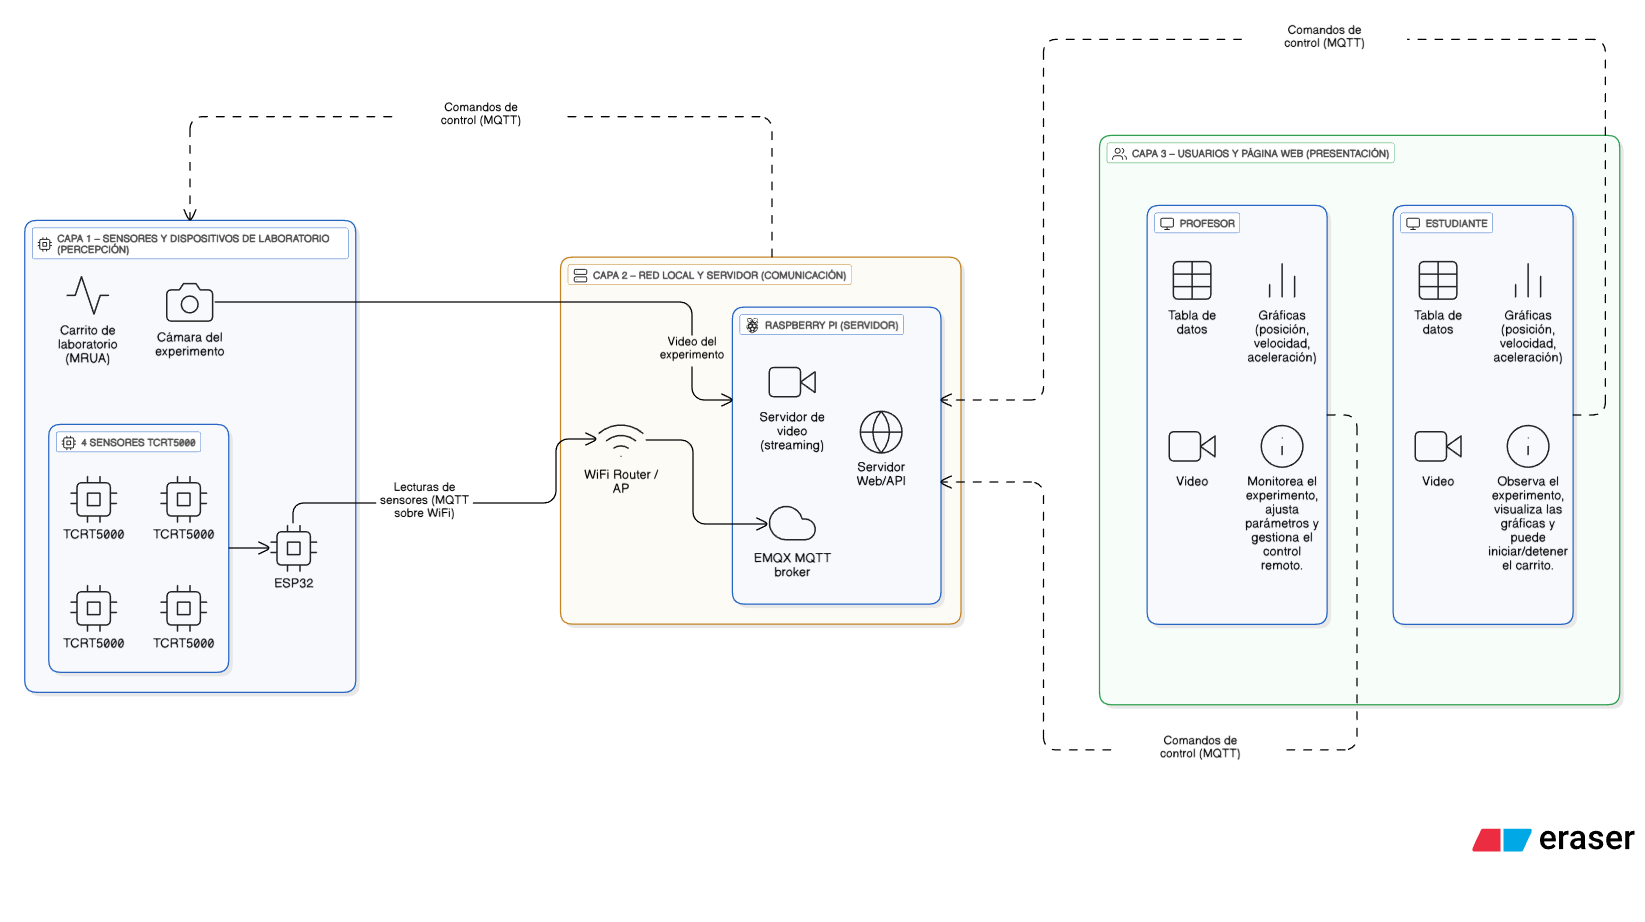
\includegraphics[width=0.88\textwidth]{../figures/fig1_arquitectura_labfisica.png}
\end{figure}

\paragraph{Procesamiento Edge computing.}
Un aspecto arquitect\'onico central es la implementaci\'on del procesamiento Edge computing en la Capa~1. El m\'odulo ESP32 ejecuta localmente la detecci\'on de eventos mediante interrupciones de hardware y genera la marca temporal de cada evento \textbf{antes} de su transmisi\'on MQTT~\parencite{r12}. Este dise\~no garantiza que la latencia de red WiFi ---inherente a cualquier sistema distribuido--- afecte \'unicamente la visualizaci\'on en la interfaz web, sin degradar la precisi\'on de las marcas temporales f\'isicas registradas, principio que sustenta la equivalencia experimental entre modalidades.

La Figura~\ref{fig:hardware_connection} muestra el diagrama de conexiones del m\'odulo de control, detallando las conexiones entre el ESP32, los sensores infrarrojos, el servomotor, el driver L298N, la pantalla LCD y el bot\'on de inicio.

\begin{figure}[htbp]
\centering
\caption{Esquem\'atico del m\'odulo de control ESP32. Se observan las conexiones a los cuatro sensores infrarrojos (GPIO~15, 25, 12, 13), el servomotor (GPIO~5), el driver L298N y la pantalla LCD v\'ia I\textsuperscript{2}C. Imagen generada con asistencia de ChatGPT~\parencite{r50}.}
\label{fig:hardware_connection}
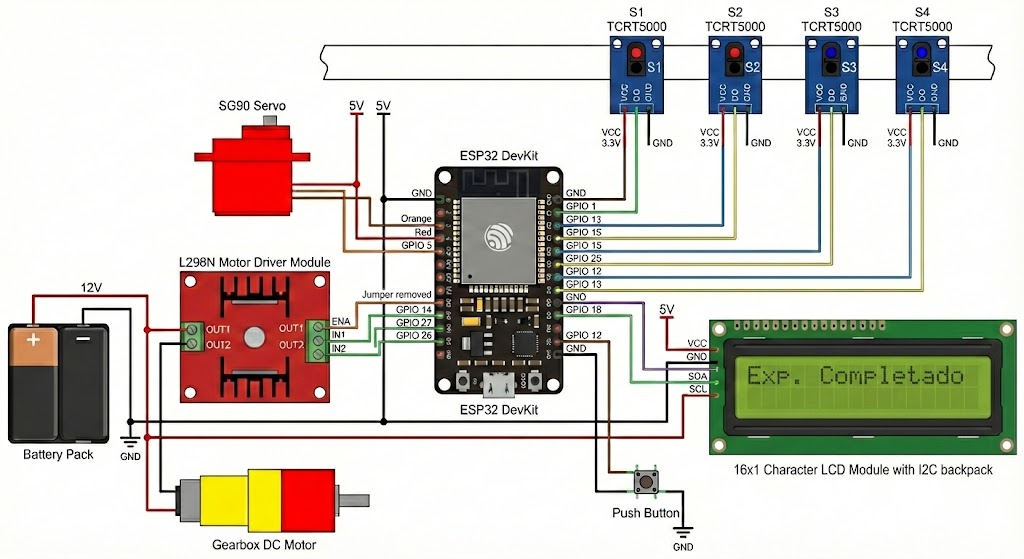
\includegraphics[width=0.88\textwidth]{../figures/Hardware connection diagram of the proposed prototype.png.jpg}
\end{figure}

\subsection{Entorno experimental y procedimiento}

El n\'umero de ensayos por modalidad ($n = 35$) fue determinado mediante an\'alisis de potencia estad\'istica \textit{a priori}. Considerando un nivel de significancia $\alpha = 0{,}05$, una potencia estad\'istica $1-\beta = 0{,}80$, y un tama\~no de efecto esperado $d = 0{,}5$~\parencite{cohen1988} para la detecci\'on de diferencias medias entre modalidades, el an\'alisis indica un tama\~no m\'inimo de $n = 26$ por grupo. Se adopt\'o $n = 35$ para aumentar la potencia efectiva a $\approx 0{,}90$ y proporcionar mayor robustez ante posibles ensayos inv\'alidos.

El experimento se llev\'o a cabo en el laboratorio de f\'isica de la PUCE sede Esmeraldas. La pista Hot Wheels\textsuperscript{\textregistered}~\parencite{r18} de 160~cm de longitud efectiva fue montada con los cuatro sensores infrarrojos a intervalos fijos de 53{,}2~cm. El punto de partida del carrito, la inclinaci\'on de la pista y las posiciones de los sensores se mantuvieron constantes en todos los ensayos para garantizar la comparabilidad entre modalidades. La pista fue inclinada a un \'angulo de $\theta = 5{,}4\degree$ respecto a la horizontal, determinado mediante un inclin\'ometro digital con resoluci\'on de $0{,}1\degree$. Este \'angulo produce una aceleraci\'on te\'orica esperada de $a_{\text{te\'orica}} = 9{,}81 \cdot \sin(5{,}4\degree) \approx 0{,}92$~m/s$^2$, valor consistente con la aceleraci\'on experimental media obtenida ($\mu \approx 0{,}95$~m/s$^2$, diferencia relativa del 3{,}3\%).

Se ejecutaron 70 ensayos distribuidos en dos modalidades: (1)~\textbf{modalidad remota}, en la que el operador activaba el experimento a trav\'es de la interfaz web y los tiempos de detecci\'on eran registrados autom\'aticamente por el sistema IoT; (2)~\textbf{modalidad presencial}, utilizando el mismo montaje f\'isico y m\'odulo ESP32 sin el componente de interfaz remota, que sirvi\'o como l\'inea base de referencia. El flujo completo de datos durante la operaci\'on se ilustra en la Figura~\ref{fig:flujo-datos}.

\begin{figure}[htbp]
\centering
\caption{Flujo de datos durante la operaci\'on del sistema. Las marcas temporales generadas por el ESP32 son publicadas v\'ia MQTT al servidor Raspberry Pi, procesadas por el backend y expuestas a la interfaz web para su visualizaci\'on en tiempo real~\parencite{r49}.}
\label{fig:flujo-datos}
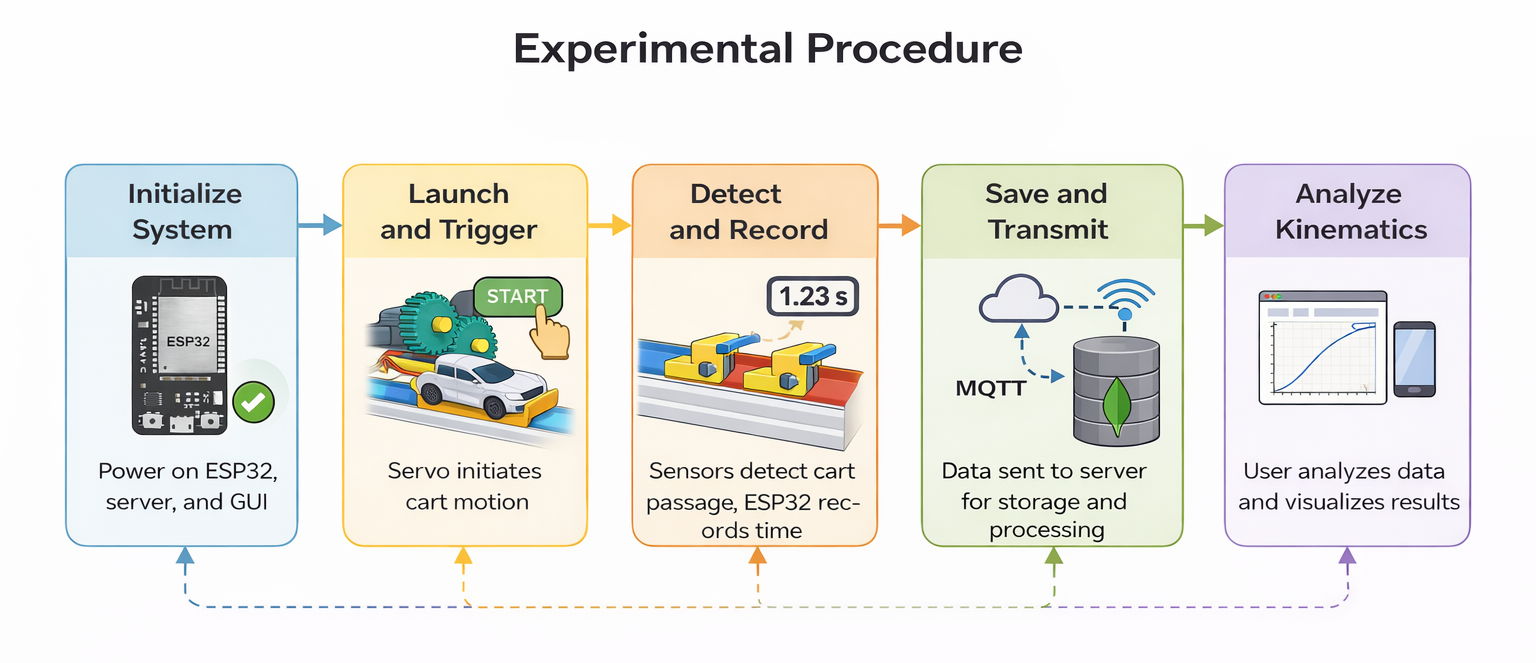
\includegraphics[width=0.88\textwidth]{../figures/Experimental procedure flowchart.png}
\end{figure}

\subsection{M\'etricas de evaluaci\'on y justificaci\'on estad\'istica}

La validaci\'on t\'ecnica del sistema se basa en tres herramientas estad\'isticas complementarias, seleccionadas por su idoneidad para el an\'alisis de equivalencia entre m\'etodos de medici\'on con muestras independientes:

La \textbf{prueba~t de Student para muestras independientes} (o su alternativa no param\'etrica de Mann--Whitney en caso de no normalidad) eval\'ua si las medias de tiempos de detecci\'on difieren significativamente entre modalidades:
\begin{equation}
  t = \frac{\bar{x}_P - \bar{y}_R}{\sqrt{\frac{s_P^2}{n_P} + \frac{s_R^2}{n_R}}}
  \label{eq:ttest}
\end{equation}
donde $\bar{x}_P$ y $\bar{y}_R$ representan las medias de tiempos de detecci\'on en la modalidad presencial y remota, respectivamente, $s_P^2$ y $s_R^2$ sus varianzas, y $n_P = n_R = 35$ el n\'umero de ensayos por modalidad.

La \textbf{prueba de Levene} contrasta la igualdad de varianzas entre modalidades, permitiendo determinar si la dispersi\'on de los datos es estad\'isticamente equivalente.

El \textbf{an\'alisis de Bland--Altman}~\parencite{bland1986} cuantifica el nivel de acuerdo cl\'inico-instrumental entre ambas modalidades y detecta posibles sesgos sistem\'aticos. Este m\'etodo calcula la diferencia media ($\overline{d}$) entre modalidades y los l\'imites de concordancia al 95\% ($\overline{d} \pm 1{,}96\,\sigma_d$), siendo especialmente adecuado para evaluar la equivalencia entre m\'etodos de medici\'on cl\'inicos e instrumentales~\parencite{giavarina2015}.

La combinaci\'on de estas tres herramientas proporciona evidencia multidimensional de equivalencia experimental: la prueba~t verifica la igualdad de medias, la prueba de Levene verifica la igualdad de varianzas, y el an\'alisis Bland--Altman detecta sesgos sistem\'aticos y cuantifica el acuerdo global.

%========================================================
\section{Resultados y discusi\'on}

\subsection{Montaje experimental implementado}

La Figura~\ref{fig:montaje_detalles} presenta la implementaci\'on f\'isica del prototipo. El sistema de detecci\'on consta de cuatro sensores infrarrojos distribuidos a intervalos de 53{,}2~cm, integrados a lo largo de la estructura para capturar el tiempo total desde la liberaci\'on automatizada del carrito hasta el final del recorrido. La interfaz web de control remoto se muestra en la Figura~\ref{fig:interfaz_web}; esta plataforma centraliza el control del experimento, procesa los datos en tiempo real y genera autom\'aticamente gr\'aficas cinem\'aticas tras cada ensayo, garantizando al mismo tiempo la supervisi\'on visual del proceso mediante transmisi\'on de video en vivo.

\begin{figure}[htbp]
\centering
\caption{Vista general del montaje experimental del sistema de MRUA con \textit{retrofitting} IoT. Se observan la pista de 160~cm, los cuatro sensores infrarrojos en sus soportes impresos en 3D, el servomotor de liberaci\'on y el m\'odulo de control ESP32.}
\label{fig:montaje_detalles}
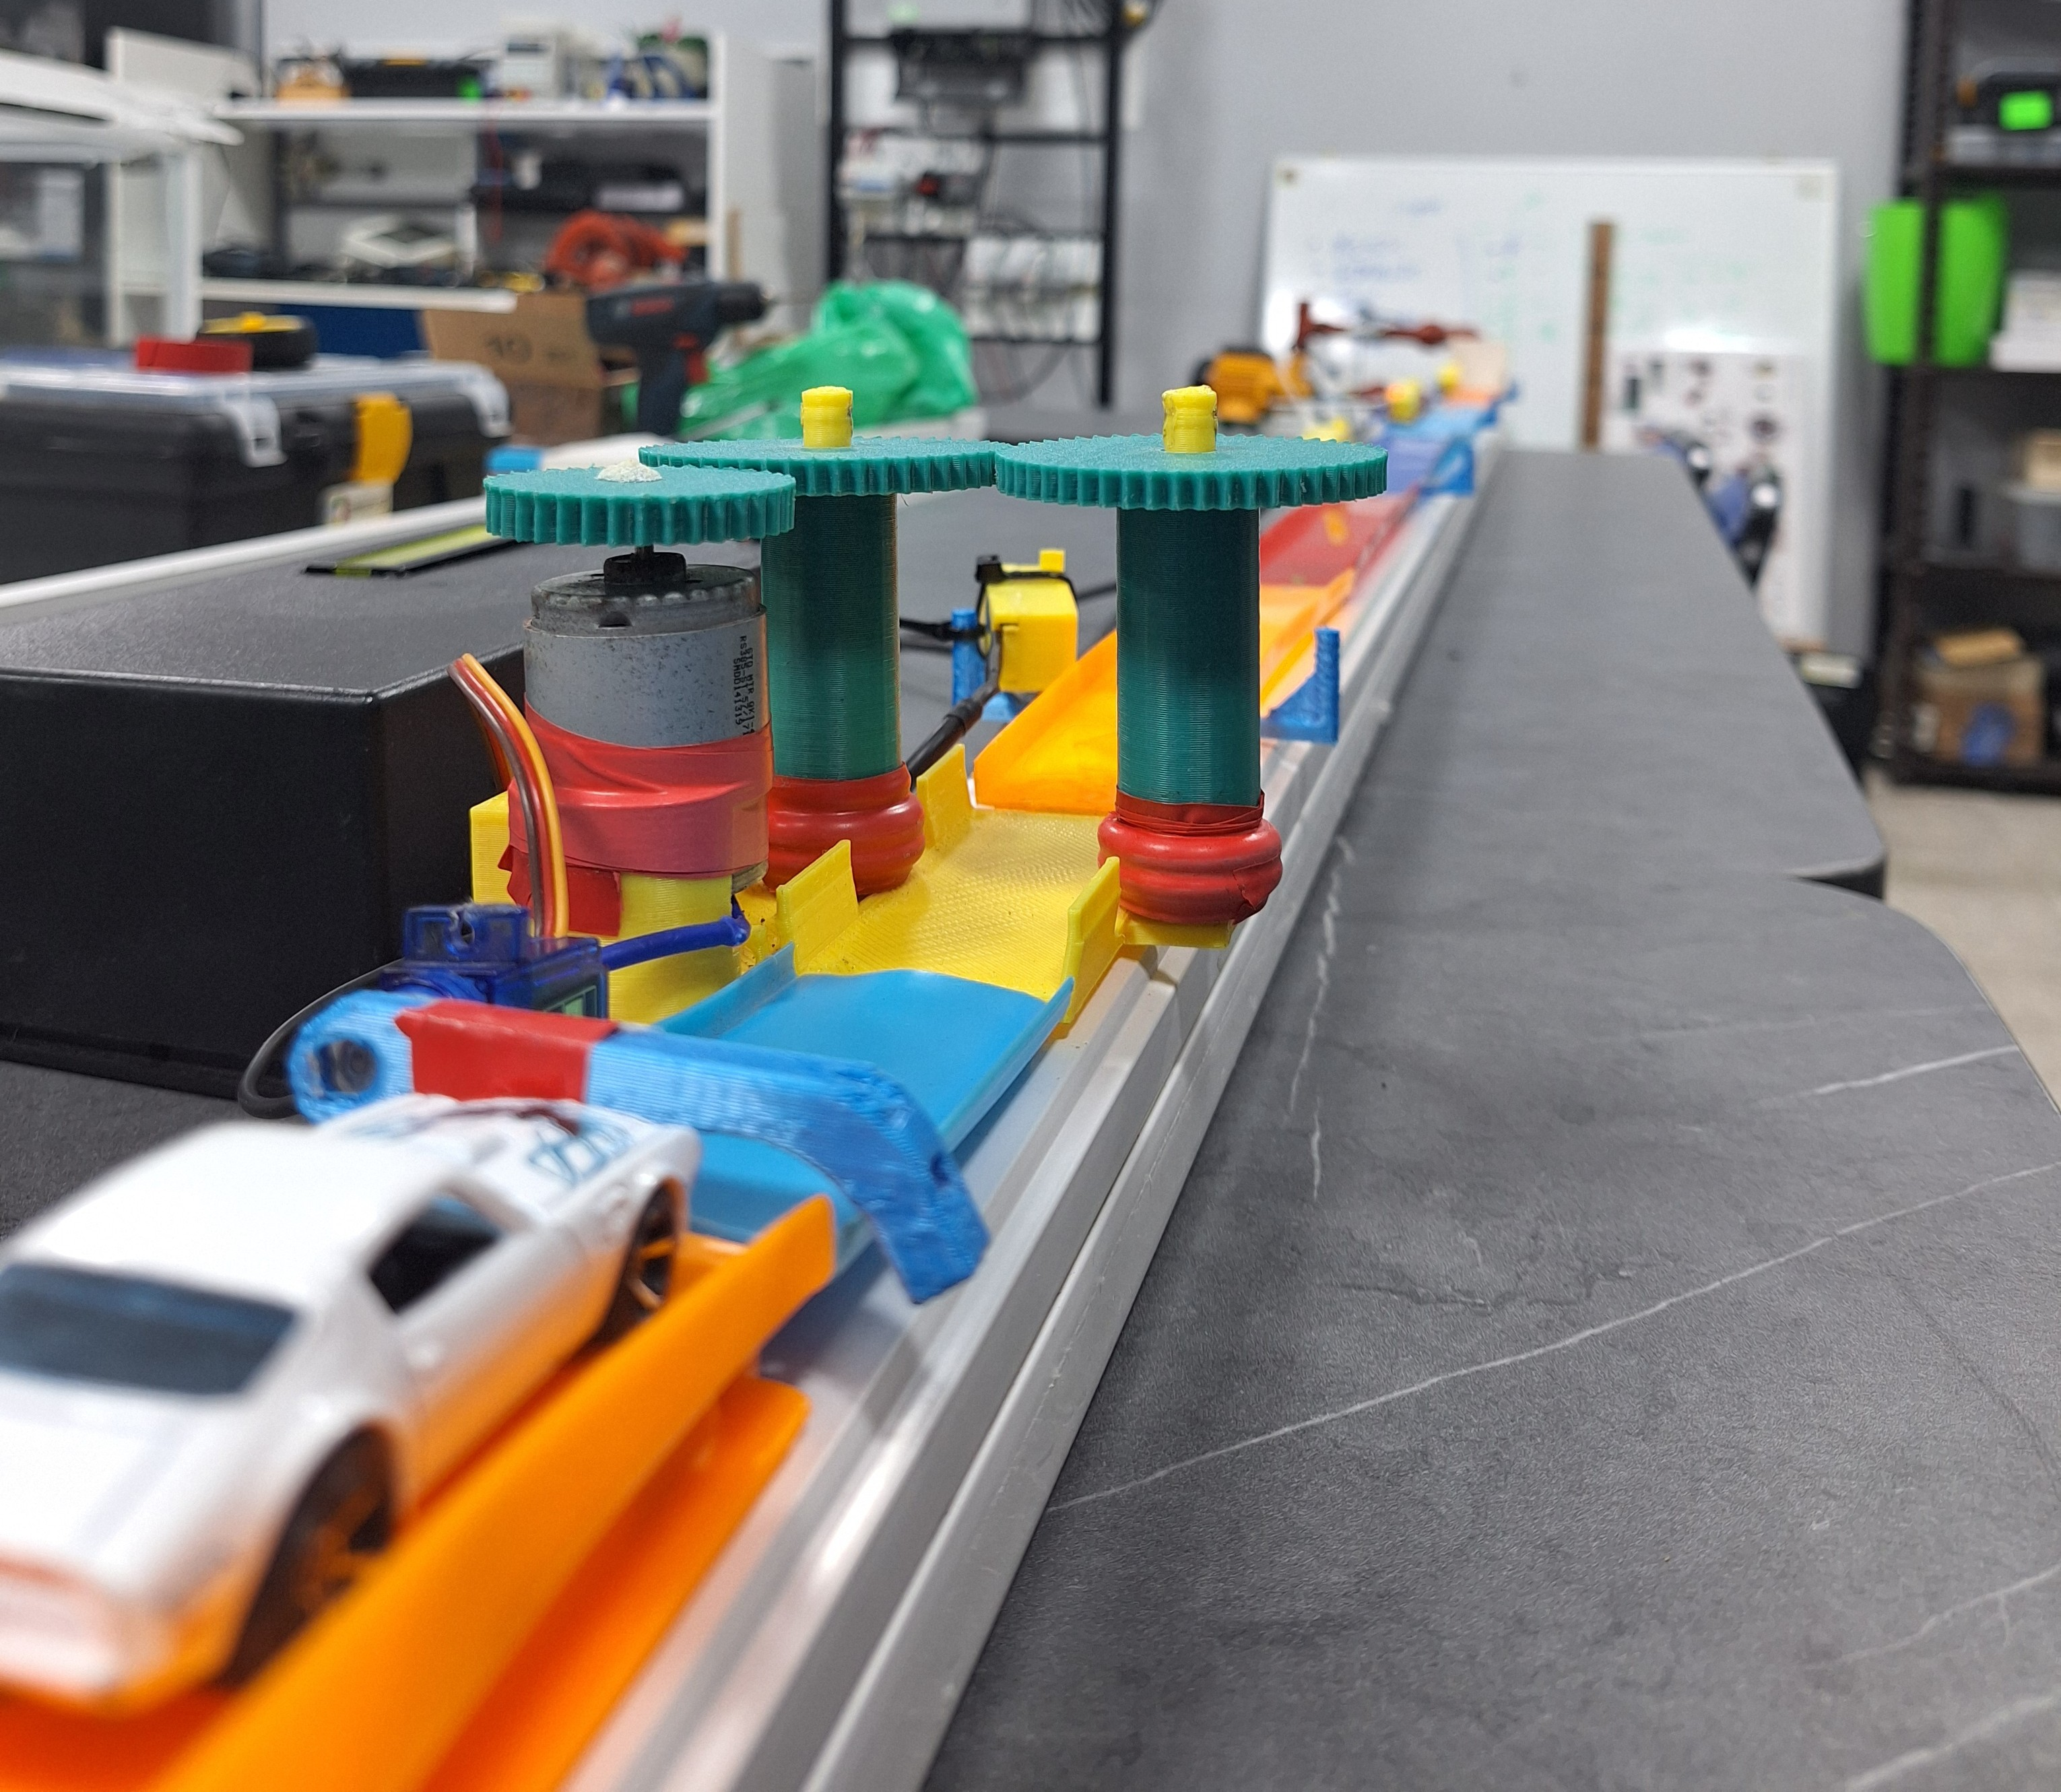
\includegraphics[width=0.88\textwidth]{../figures/setup_overview_completo.jpg}
\end{figure}

\begin{figure}[htbp]
\centering
\caption{Interfaz web desarrollada para el control y monitoreo remoto del experimento. La plataforma permite iniciar y detener la secuencia experimental, visualizar los resultados cinem\'aticos generados autom\'aticamente y supervisar el movimiento del carrito mediante video en tiempo real.}
\label{fig:interfaz_web}
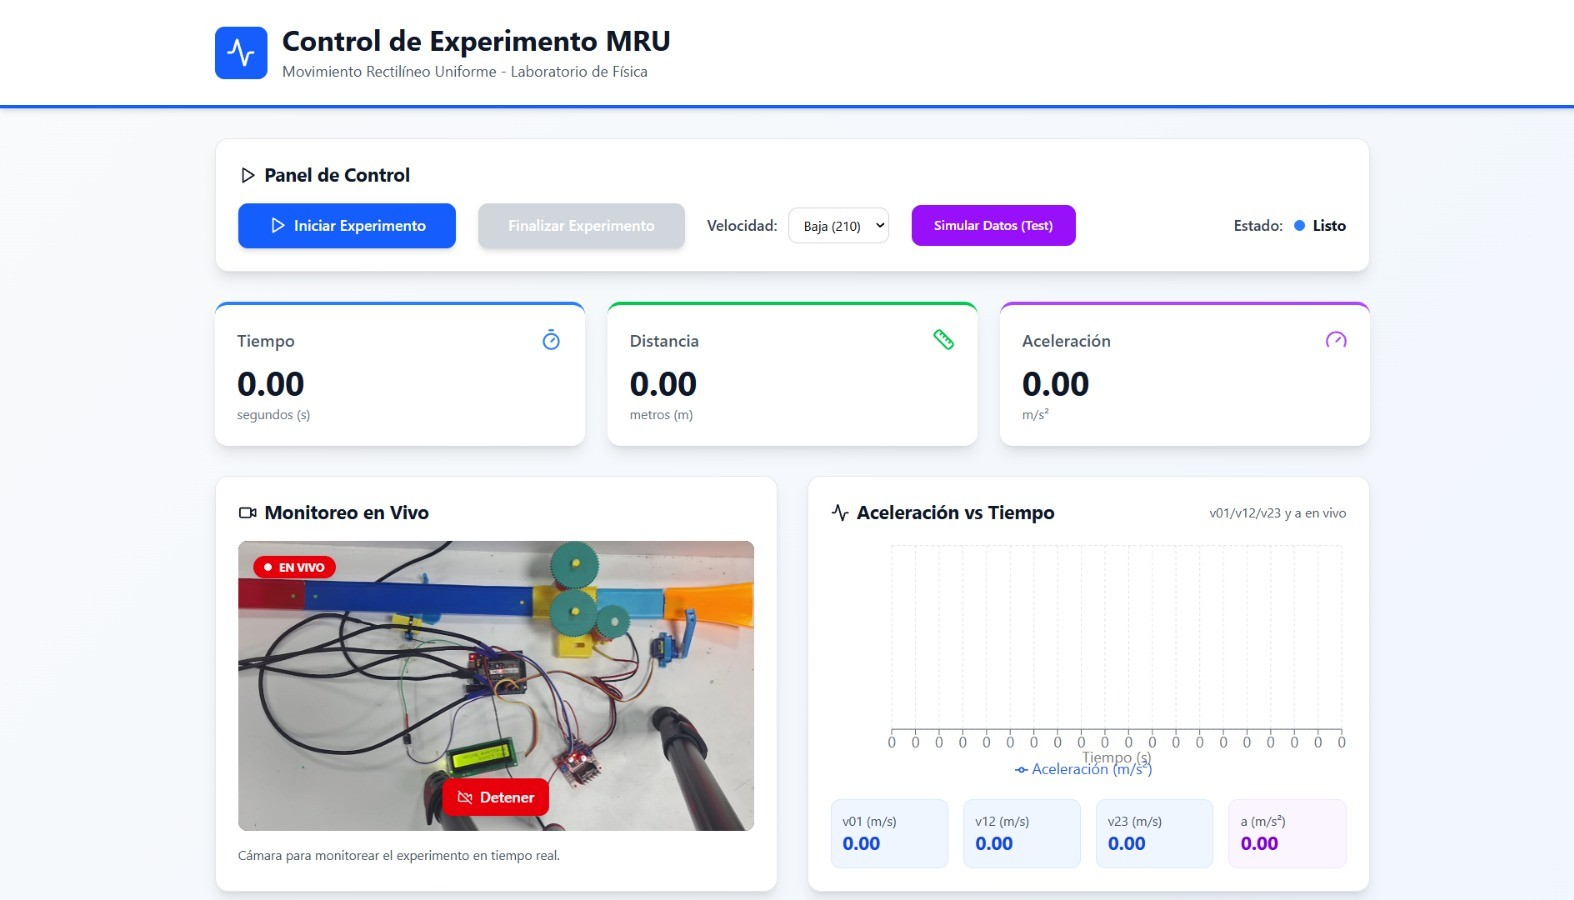
\includegraphics[width=0.88\textwidth]{../figures/InterfazWeb.jpg}
\end{figure}

\subsection{Resumen estad\'istico global}

La Tabla~\ref{tab:resumen_global} sintetiza los resultados estad\'isticos comparativos por sensor. La normalidad de las distribuciones de tiempos fue verificada mediante la prueba de Shapiro--Wilk ($p > 0{,}05$ en todos los casos), justificando el uso de pruebas param\'etricas. La prueba de Levene confirm\'o la igualdad de varianzas entre modalidades para todos los sensores activos ($p > 0{,}05$; S2: $p = 0{,}71$; S3: $p = 0{,}89$; S4: $p = 0{,}93$). La diferencia pr\'acticamente nula entre las medias de ambas modalidades ($\Delta\bar{x} < 0{,}01$~s en todos los sensores) y la m\'inima variaci\'on en la desviaci\'on est\'andar ($\Delta\sigma < 0{,}02$~s) indican que el sistema IoT reproduce con alta fidelidad las mediciones temporales del montaje presencial de referencia. Estos valores demuestran que la latencia de red no introdujo distorsiones mensurables en los tiempos de detecci\'on, lo cual valida la efectividad del procesamiento Edge computing implementado.

\begin{table}[htbp]
\caption{Resumen estad\'istico comparativo por sensor: modalidad presencial (P) vs. remota (R), $n = 35$ por modalidad. $\Delta\bar{x}$: diferencia de medias; $\Delta\sigma$: diferencia de desviaciones est\'andar; $p$: valor~p de la prueba~t para muestras independientes. \'Angulo de inclinaci\'on: $\theta = 5{,}4\degree$; aceleraci\'on te\'orica: $a_{\text{te\'orica}} = 0{,}92$~m/s$^2$; desviaci\'on experimental: 3{,}3\%.}
\label{tab:resumen_global}
\centering
\scriptsize
\begin{tabular}{lrrrrrrrr}
\toprule
\textbf{Sensor} & $\bar{x}_P$ (s) & $\bar{y}_R$ (s) & $\Delta\bar{x}$ (s) & $\sigma_P$ (s) & $\sigma_R$ (s) & $\Delta\sigma$ (s) & $p$ & \textbf{Equiv.} \\
\midrule
S1 (ref.) & 0{,}000 & 0{,}000 & 0{,}000 & 0{,}000 & 0{,}000 & 0{,}000 & {---} & {---} \\
S2        & 1{,}09  & 1{,}09  & 0{,}00  & 0{,}15  & 0{,}16  & 0{,}01  & 0{,}98 & S\'i \\
S3        & 1{,}54  & 1{,}54  & 0{,}00  & 0{,}22  & 0{,}22  & 0{,}00  & 0{,}97 & S\'i \\
S4        & 1{,}89  & 1{,}89  & 0{,}00  & 0{,}27  & 0{,}27  & 0{,}00  & 0{,}96 & S\'i \\
\bottomrule
\end{tabular}
\end{table}

\subsection{An\'alisis de concordancia Bland--Altman}

El an\'alisis de Bland--Altman~\parencite{bland1986} se aplic\'o a los sensores activos S2, S3 y S4. Los resultados (Tabla~\ref{tab:bland_altman} y Figura~\ref{fig:bland_altman}) revelan que el sesgo medio ($\overline{d}$) es pr\'acticamente nulo en todos los puntos de medici\'on ($|\overline{d}| < 0{,}002$~s), lo cual constituye la evidencia central de la \textbf{ausencia de sesgo sistem\'atico} entre modalidades. La amplitud de los l\'imites de concordancia al 95\% ($\pm$0{,}46--0{,}80~s) refleja la variabilidad f\'isica inherente a los ensayos no emparejados ---determinada por las condiciones de lanzamiento del carrito--- y no limitaciones instrumentales del sistema IoT. La consistencia de estos valores con la propagaci\'on cuadr\'atica de las desviaciones individuales ($\sigma_d \approx \sqrt{\sigma_P^2 + \sigma_R^2}$) confirma que la dispersi\'on observada tiene origen f\'isico, no instrumental.

\begin{table}[htbp]
\caption{An\'alisis Bland--Altman por sensor: $\overline{d} = \bar{x}_P - \bar{y}_R$; l\'imites de concordancia al 95\% calculados como $\overline{d} \pm 1{,}96\,\sigma_d$.}
\label{tab:bland_altman}
\centering
\scriptsize
\begin{tabular}{lcccc}
\toprule
\textbf{Sensor} & $\overline{d}$ (s) & $\sigma_d$ (s) & \textbf{L\'im. inferior (s)} & \textbf{L\'im. superior (s)} \\
\midrule
S2 & 0{,}000 & 0{,}234 & $-$0{,}459 & 0{,}460 \\
S3 & 0{,}002 & 0{,}332 & $-$0{,}649 & 0{,}653 \\
S4 & 0{,}001 & 0{,}408 & $-$0{,}799 & 0{,}800 \\
\bottomrule
\end{tabular}
\end{table}

Para evaluar la aceptabilidad de los l\'imites de concordancia, se adopta como criterio de referencia la tolerancia m\'axima instrumental definida por el objetivo did\'actico del experimento: una diferencia de $\pm 1$~s en los tiempos de detecci\'on es pedag\'ogicamente aceptable para el nivel de un curso de f\'isica de ingenier\'ia, dado que la resoluci\'on temporal relevante para distinguir reg\'imenes cinem\'aticos es del orden de d\'ecimas de segundo. Los l\'imites de concordancia obtenidos (m\'aximo $\pm 0{,}80$~s) se encuentran dentro de este umbral, confirmando la equivalencia operativa del sistema IoT para su prop\'osito educativo.

\begin{figure}[htbp]
    \centering
    \caption{An\'alisis Bland--Altman para los sensores S2, S3 y S4. La l\'inea continua central indica el sesgo medio ($\overline{d} \approx 0$); las l\'ineas punteadas delimitan los l\'imites de concordancia al 95\%. La ausencia de tendencia en la distribuci\'on de diferencias confirma que el sistema IoT no introduce sesgo sistem\'atico proporcional a la magnitud de la medici\'on. Nota: las etiquetas de la figura se presentan en ingl\'es para facilitar la difusi\'on internacional del resultado.}
    \label{fig:bland_altman}
    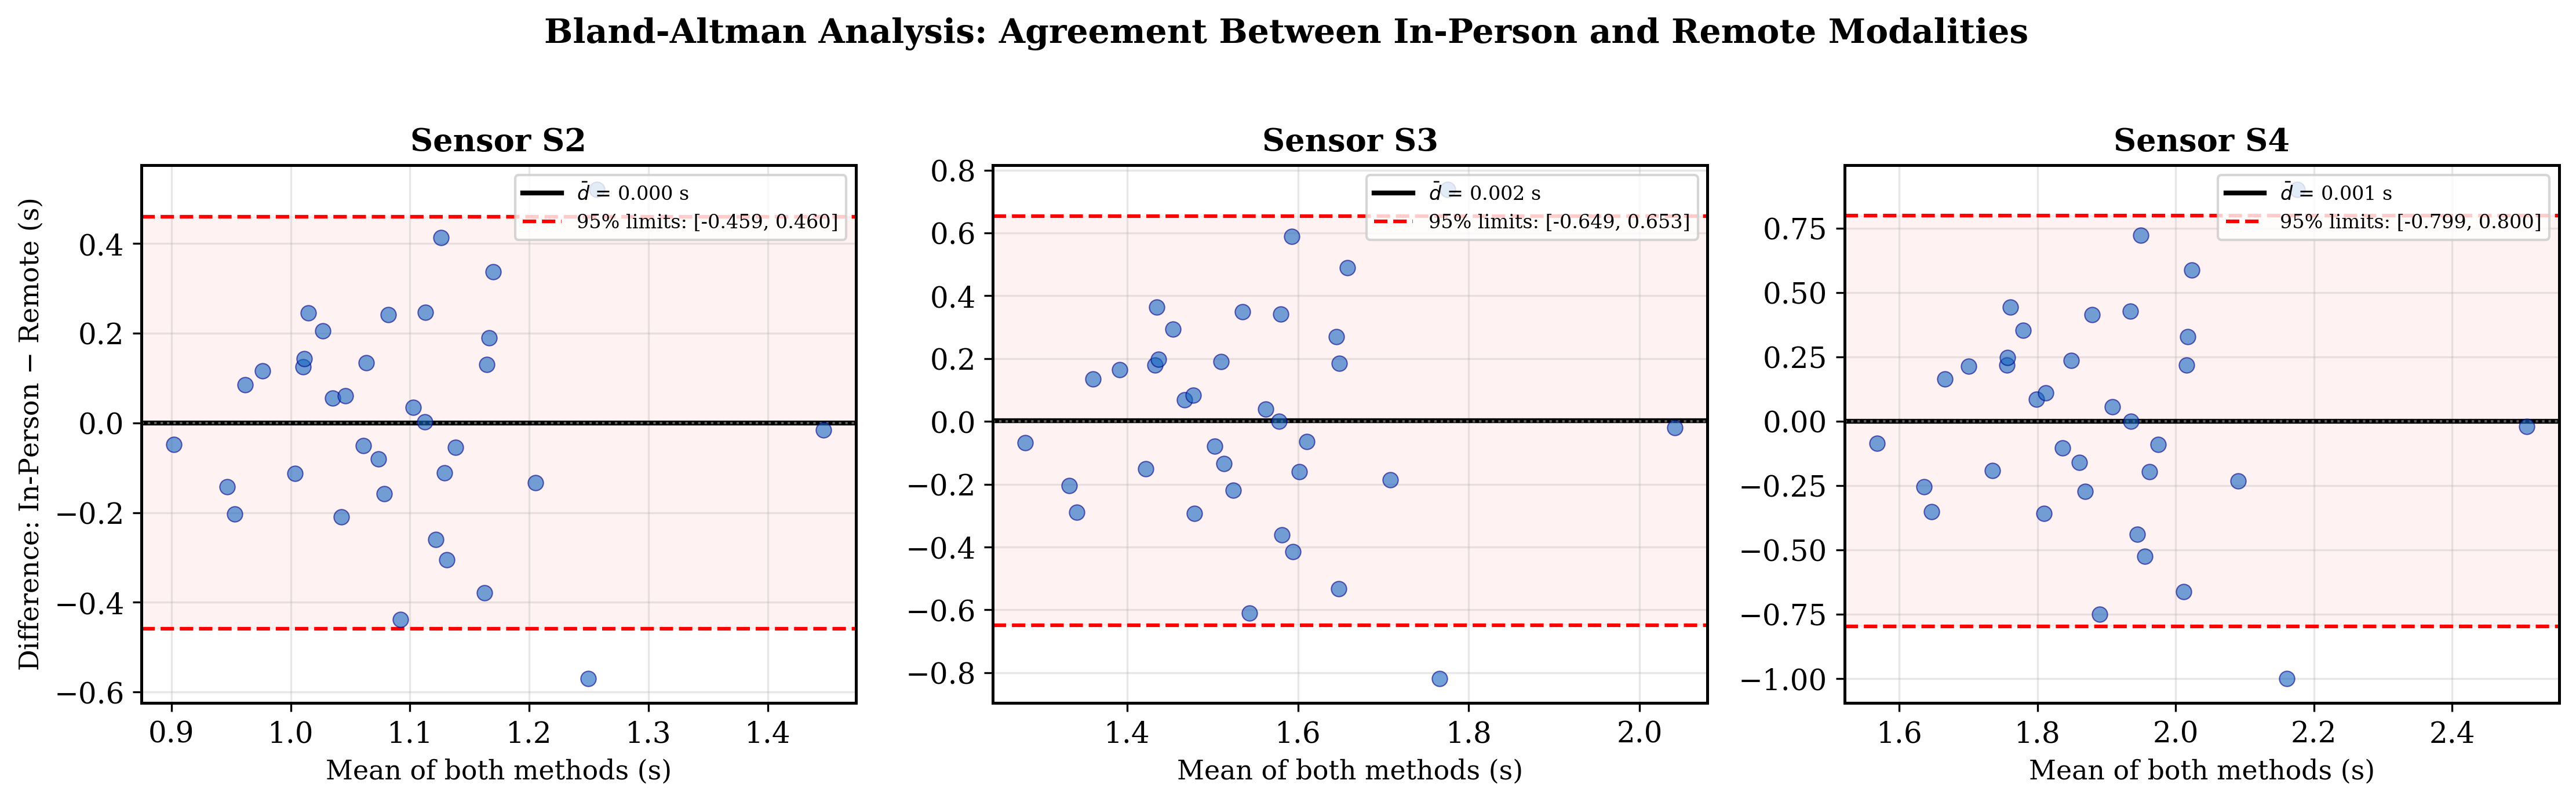
\includegraphics[width=0.88\textwidth]{../figures/bland_altman_english_white.png}
\end{figure}

\subsection{An\'alisis cinem\'atico global}

La Figura~\ref{fig:vel_profile} muestra el perfil de velocidad media para ambas modalidades. Las curvas son pr\'acticamente indistinguibles a lo largo de toda la trayectoria, lo que indica que el sistema IoT captura el comportamiento din\'amico del MRUA con una fidelidad equivalente a la del montaje presencial. Esto permite concluir que la uniformidad del incremento de velocidad entre segmentos consecutivos es coherente con el modelo te\'orico de aceleraci\'on constante (Ecuaci\'on~\ref{eq:aceleracion}).

\begin{figure}[htbp]
  \centering
  \caption{Perfil de velocidad media en funci\'on de la posici\'on del segmento para las modalidades remota (azul) y presencial (rojo). Las barras de error representan $\pm 1\sigma$. La superposici\'on de ambas curvas evidencia la equivalencia cinem\'atica entre modalidades.}
  \label{fig:vel_profile}
  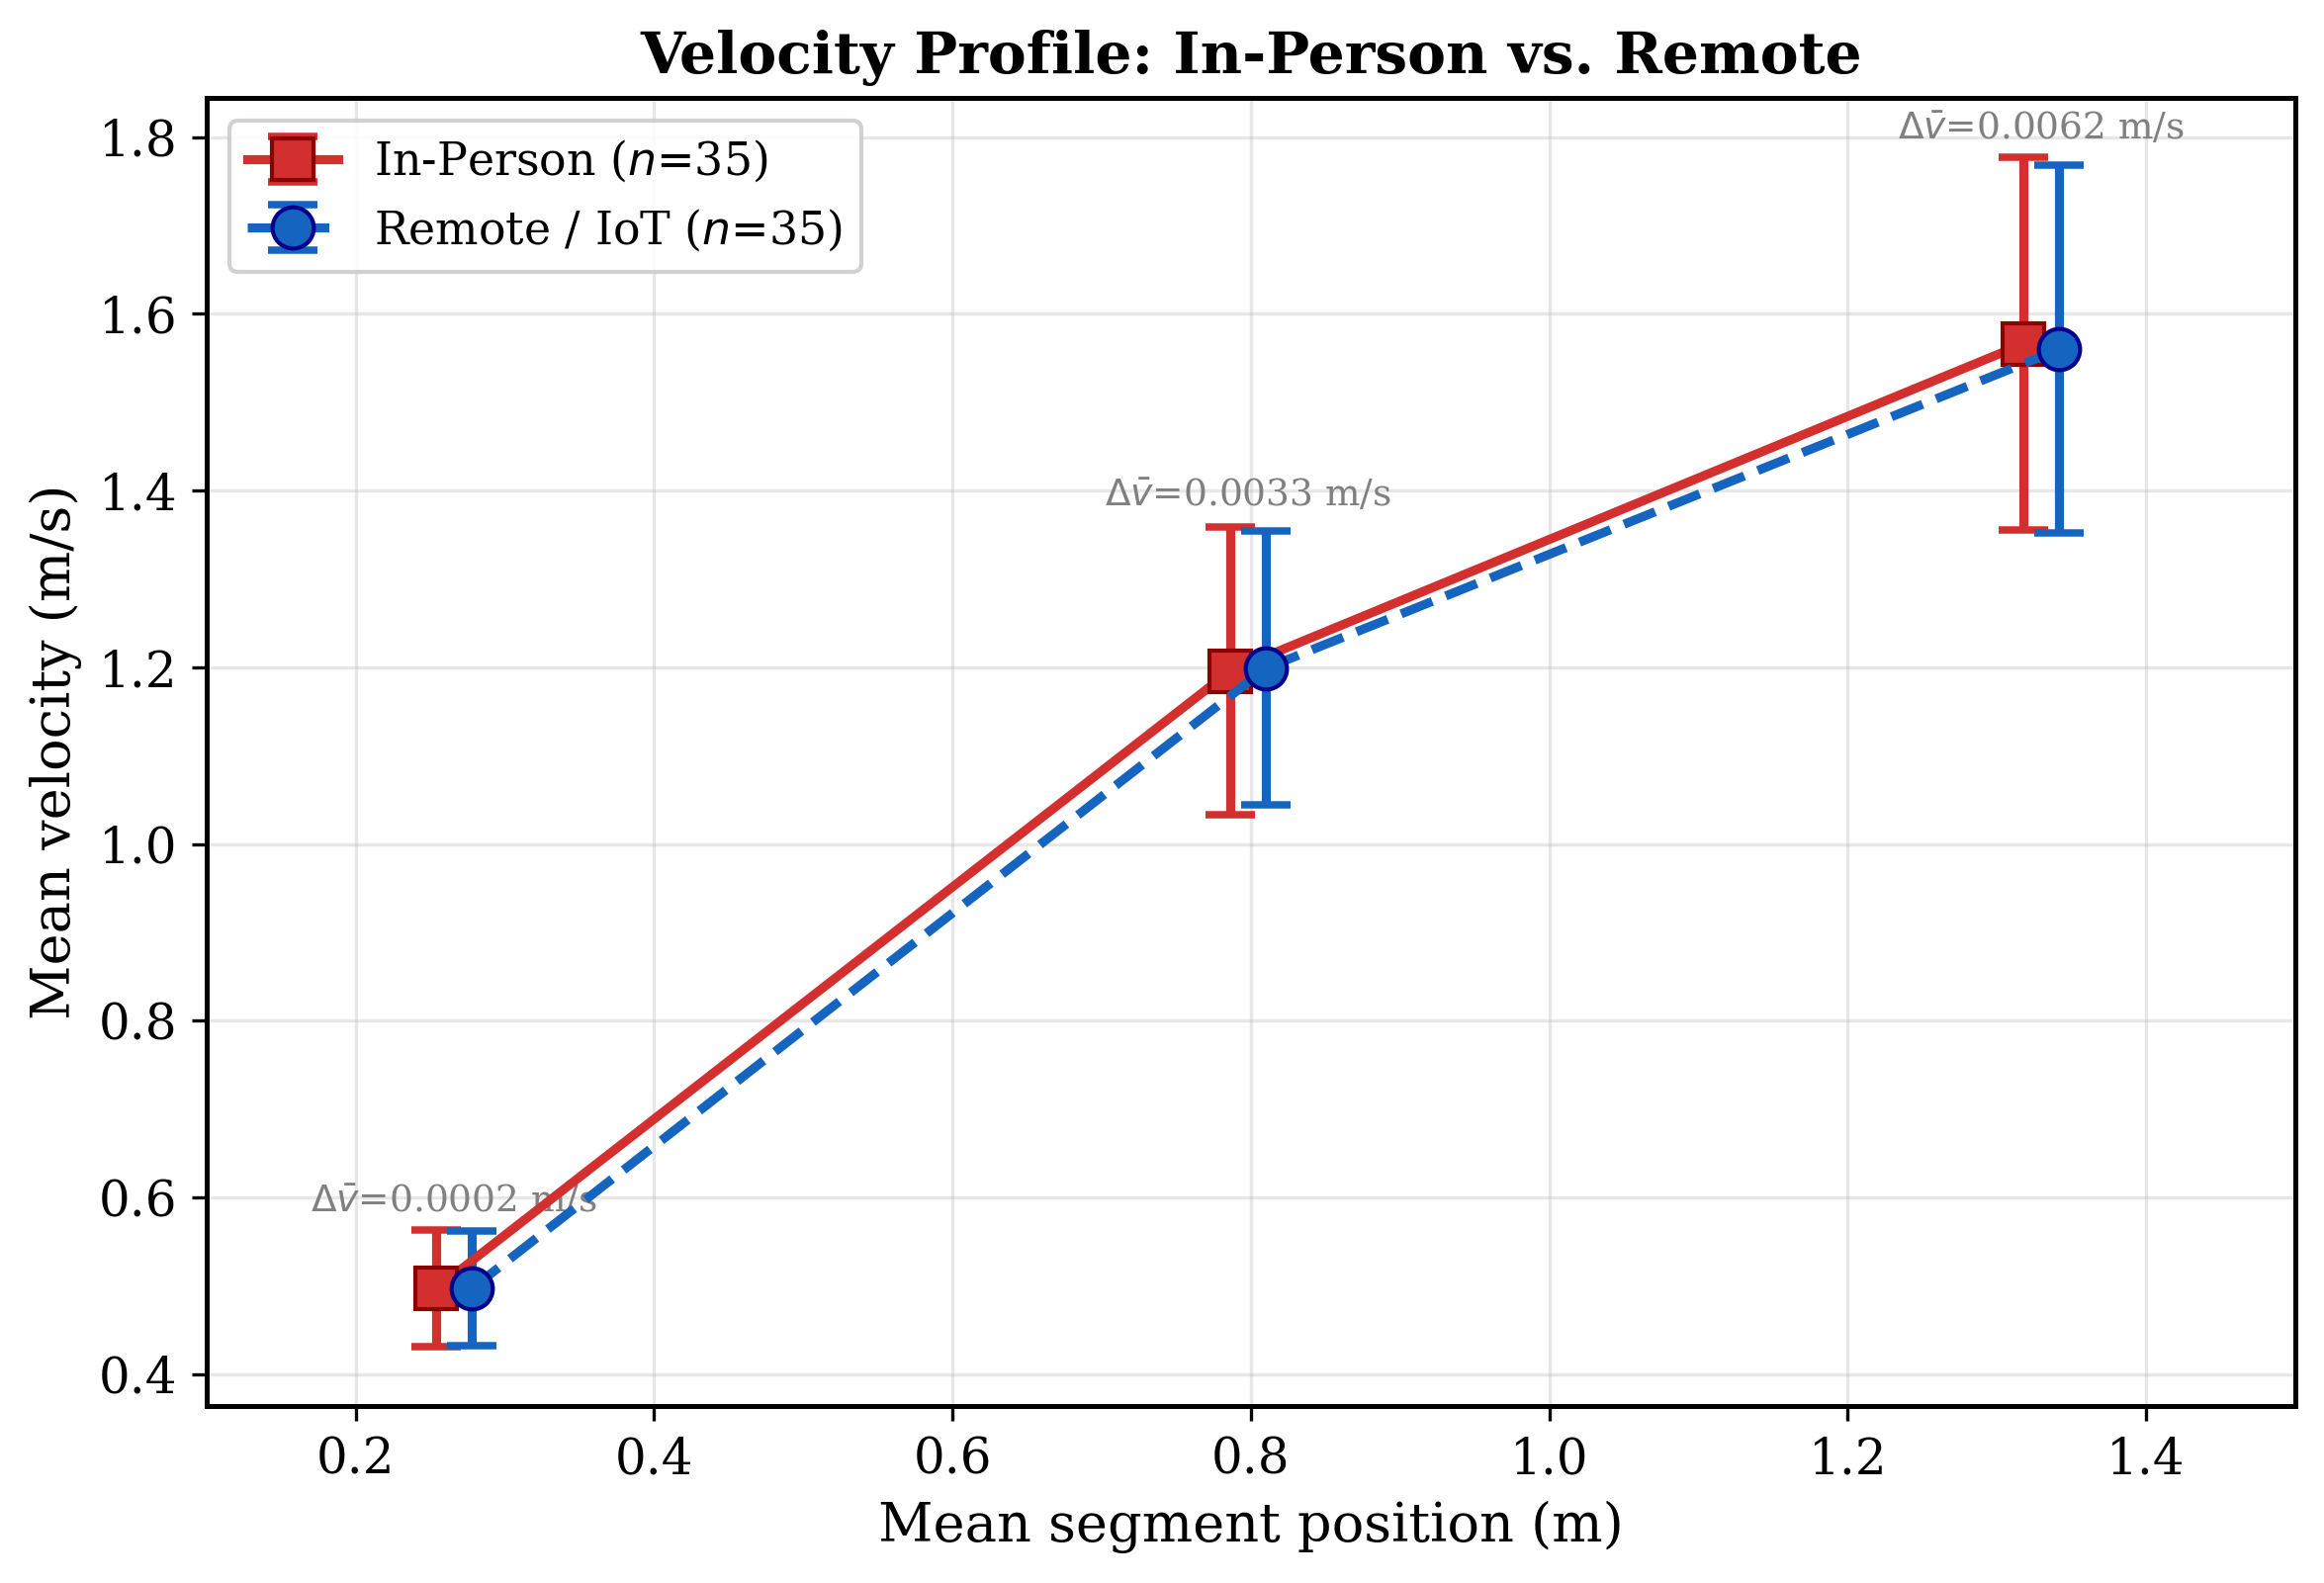
\includegraphics[width=0.88\textwidth]{../figures/velocity_profile.png}
\end{figure}

La Figura~\ref{fig:accel_box} presenta la distribuci\'on de la aceleraci\'on experimental estimada. Ambas modalidades exhiben medias id\'enticas ($\mu \approx 0{,}95$~m/s$^2$) con desviaciones est\'andar similares, lo que indica que la aceleraci\'on del MRUA es reproducida con precisi\'on equivalente en ambas modalidades. Esto permite concluir que la diferencia del 3{,}3\% respecto al valor te\'orico ($a \approx 0{,}92$~m/s$^2$, Ecuaci\'on~\ref{eq:mruateorico}) se encuentra dentro del margen de error esperado para experimentos de cinem\'atica con fricci\'on residual~\parencite{r10}, como ilustra la Figura~\ref{fig:mrua_teorico}.

\begin{figure}[htbp]
  \centering
  \caption{Distribuci\'on de la aceleraci\'on experimental estimada para las modalidades remota y presencial ($n = 35$ por modalidad). La pr\'actica identidad de medianas y rangos intercuart\'ilicos confirma la equivalencia estad\'istica entre modalidades.}
  \label{fig:accel_box}
  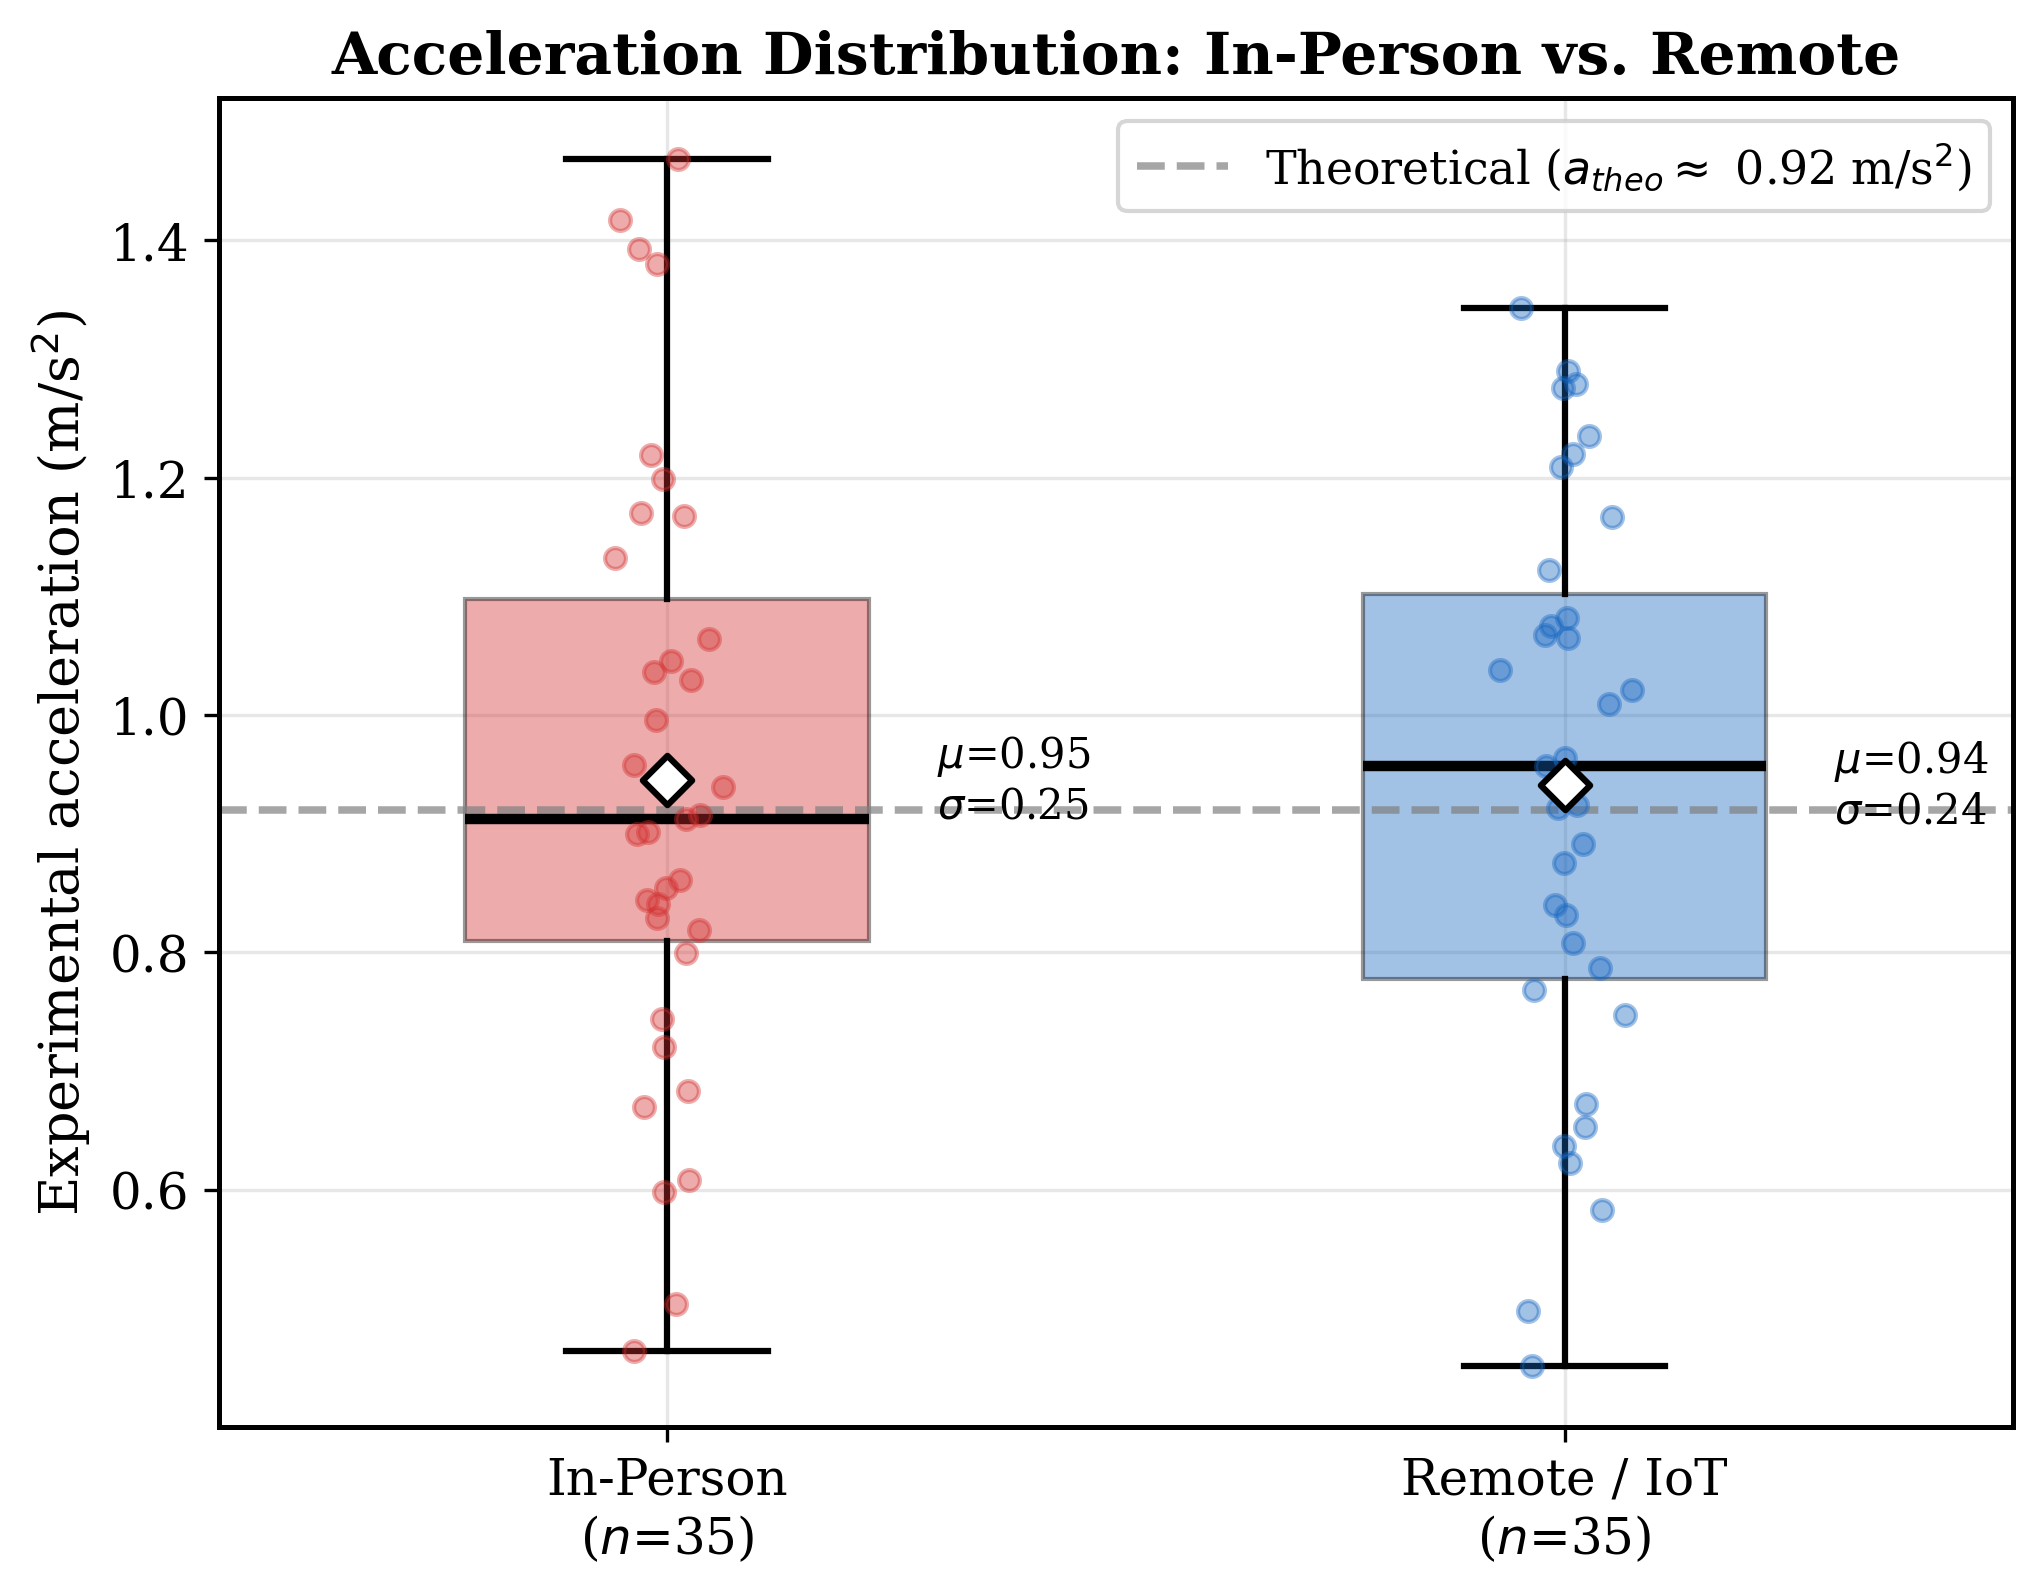
\includegraphics[width=0.65\textwidth]{../figures/acceleration_boxplot.png}
\end{figure}

\begin{figure}[htbp]
  \centering
  \caption{Posici\'on vs. tiempo: modelo te\'orico de MRUA (l\'inea gris punteada) y datos experimentales de las modalidades remota (azul) y presencial (rojo). La correspondencia entre el modelo te\'orico y los datos experimentales de ambas modalidades valida la precisi\'on del sistema de medici\'on.}
  \label{fig:mrua_teorico}
  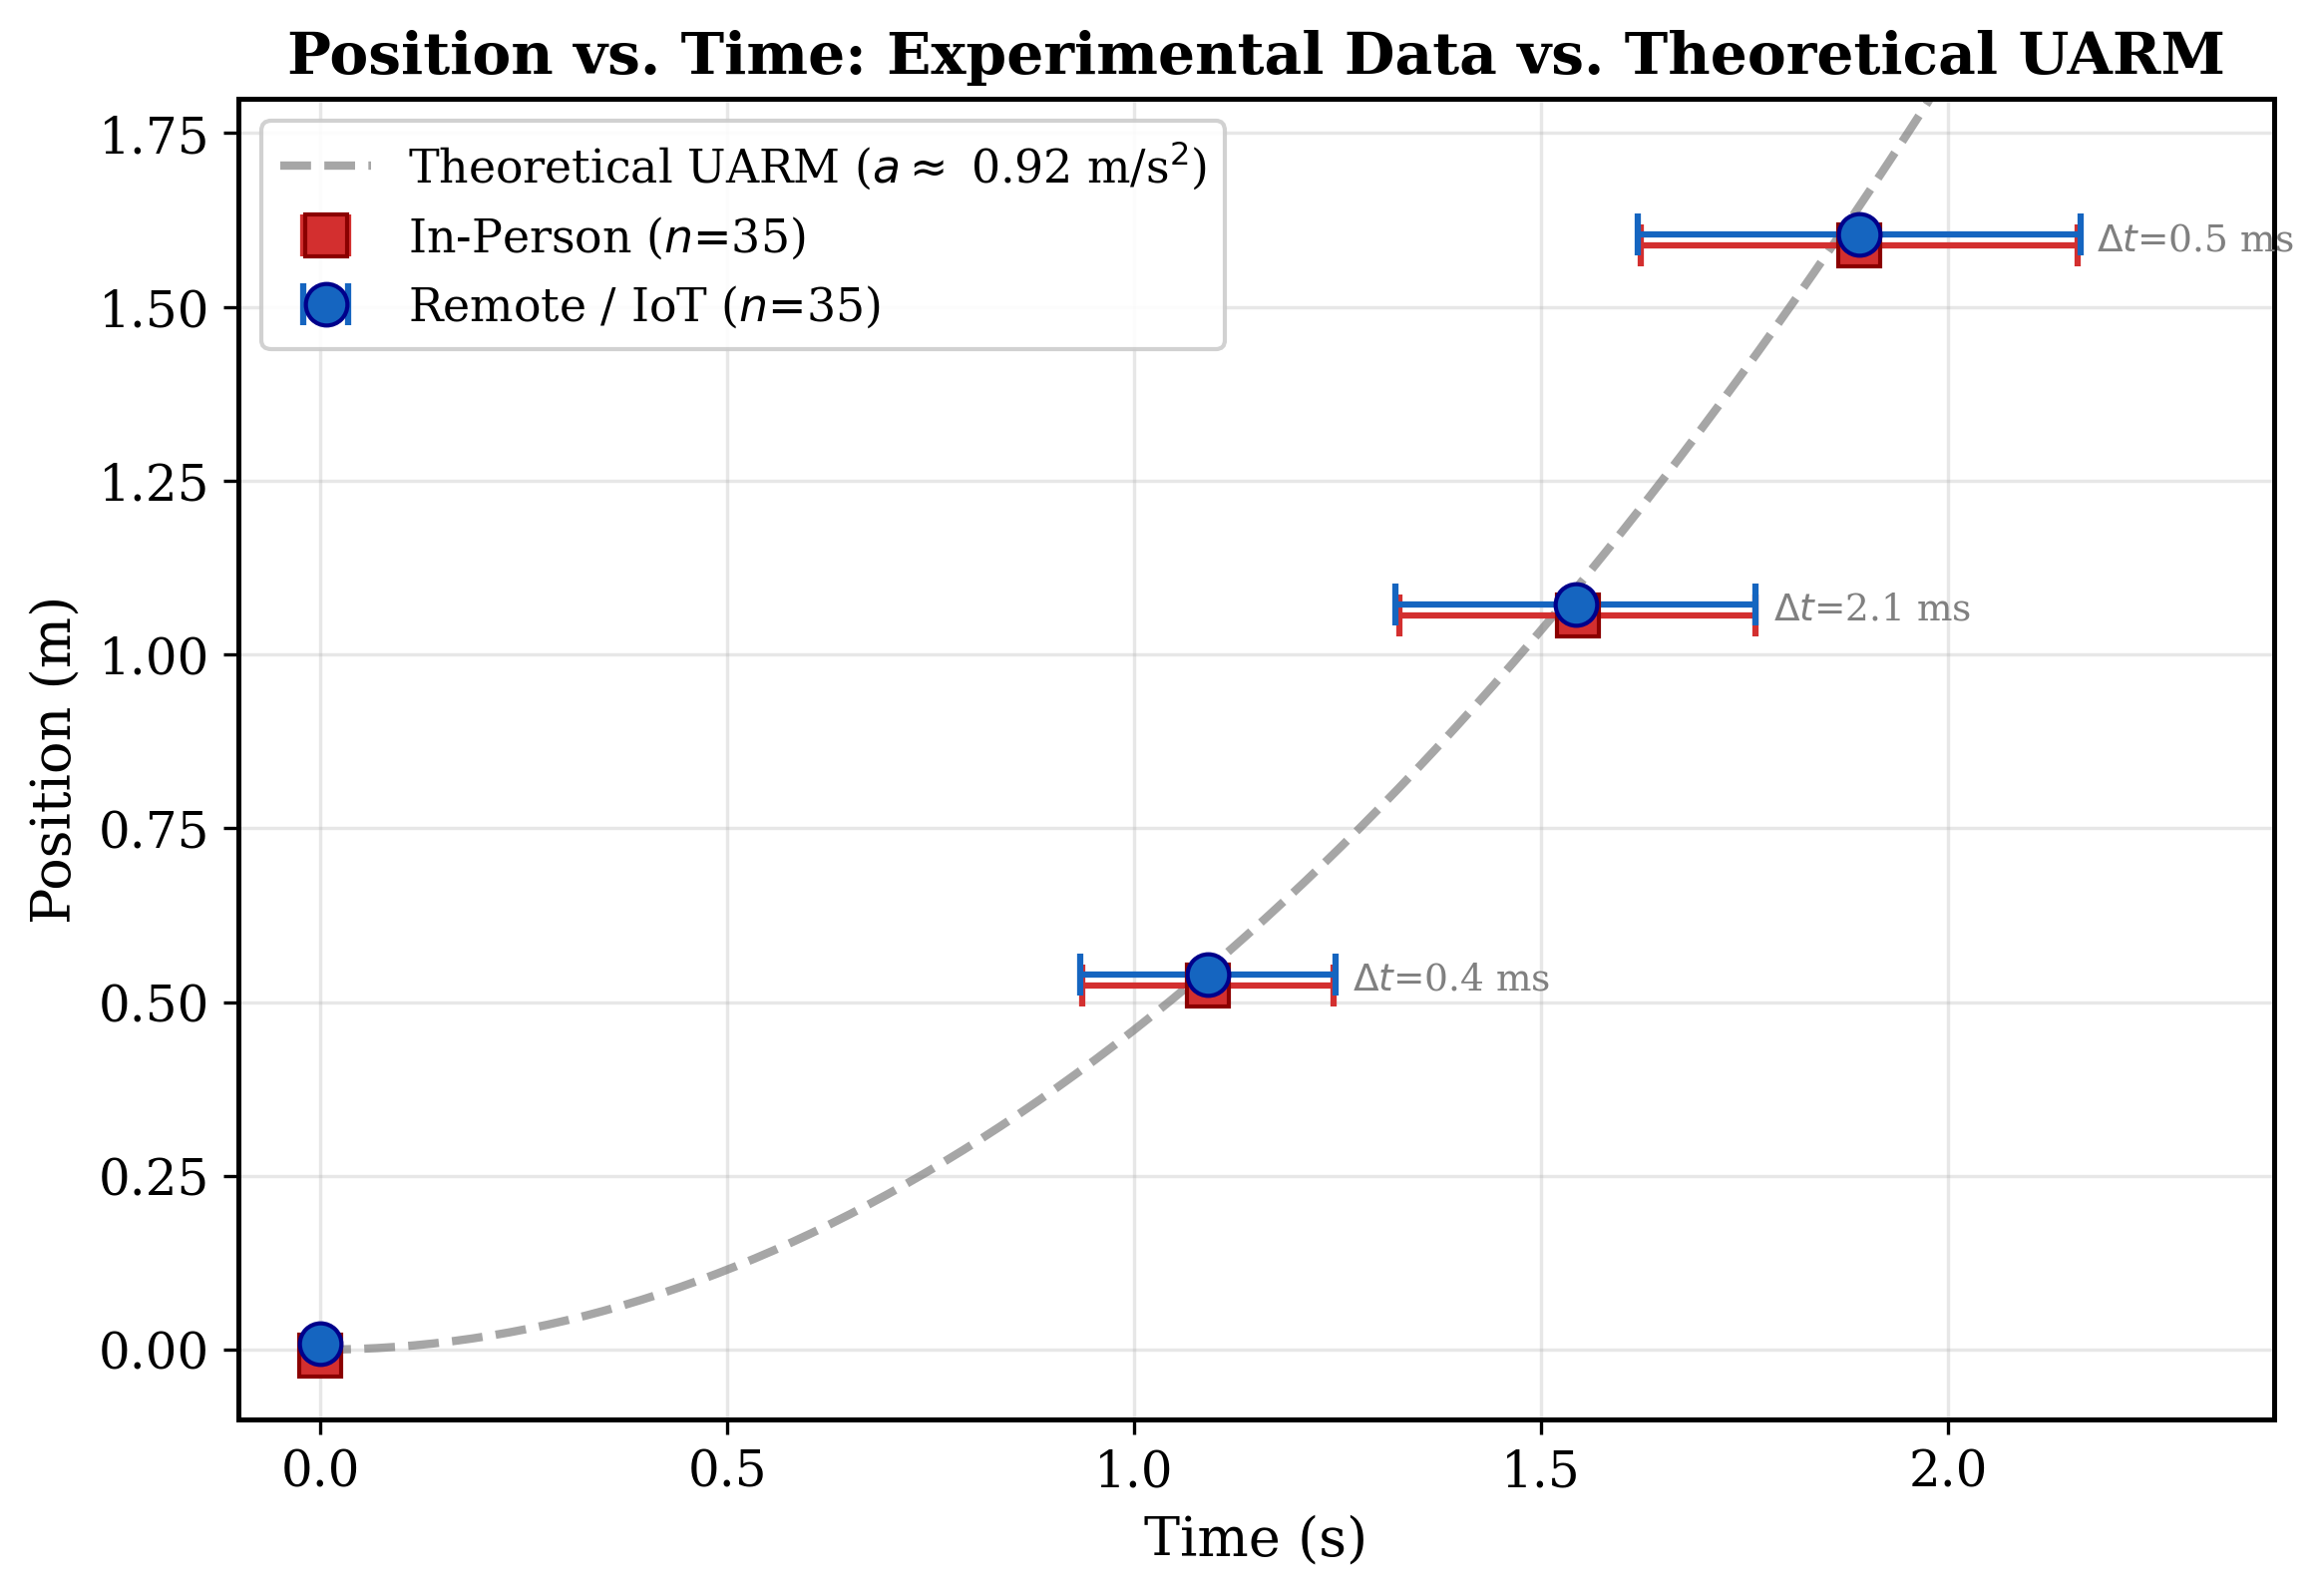
\includegraphics[width=0.88\textwidth]{../figures/experimental_vs_theoretical_mrua.png}
\end{figure}

La tasa de captura exitosa de eventos fue del 98{,}5\% en modalidad remota (Figura~\ref{fig:stability}), con una \'unica p\'erdida atribuible a una desconexi\'on moment\'anea de WiFi. Este resultado confirma la alta confiabilidad operativa del sistema bajo condiciones de red est\'andar.

\begin{figure}[H]
  \centering
  \caption{Tasa de captura exitosa de eventos: remoto (98{,}5\%) vs. presencial (100{,}0\%). La diferencia de 1{,}5\% corresponde a una sola p\'erdida de evento en la modalidad remota, atribuible a una desconexi\'on moment\'anea de red y no a una limitaci\'on estructural del sistema.}
  \label{fig:stability}
  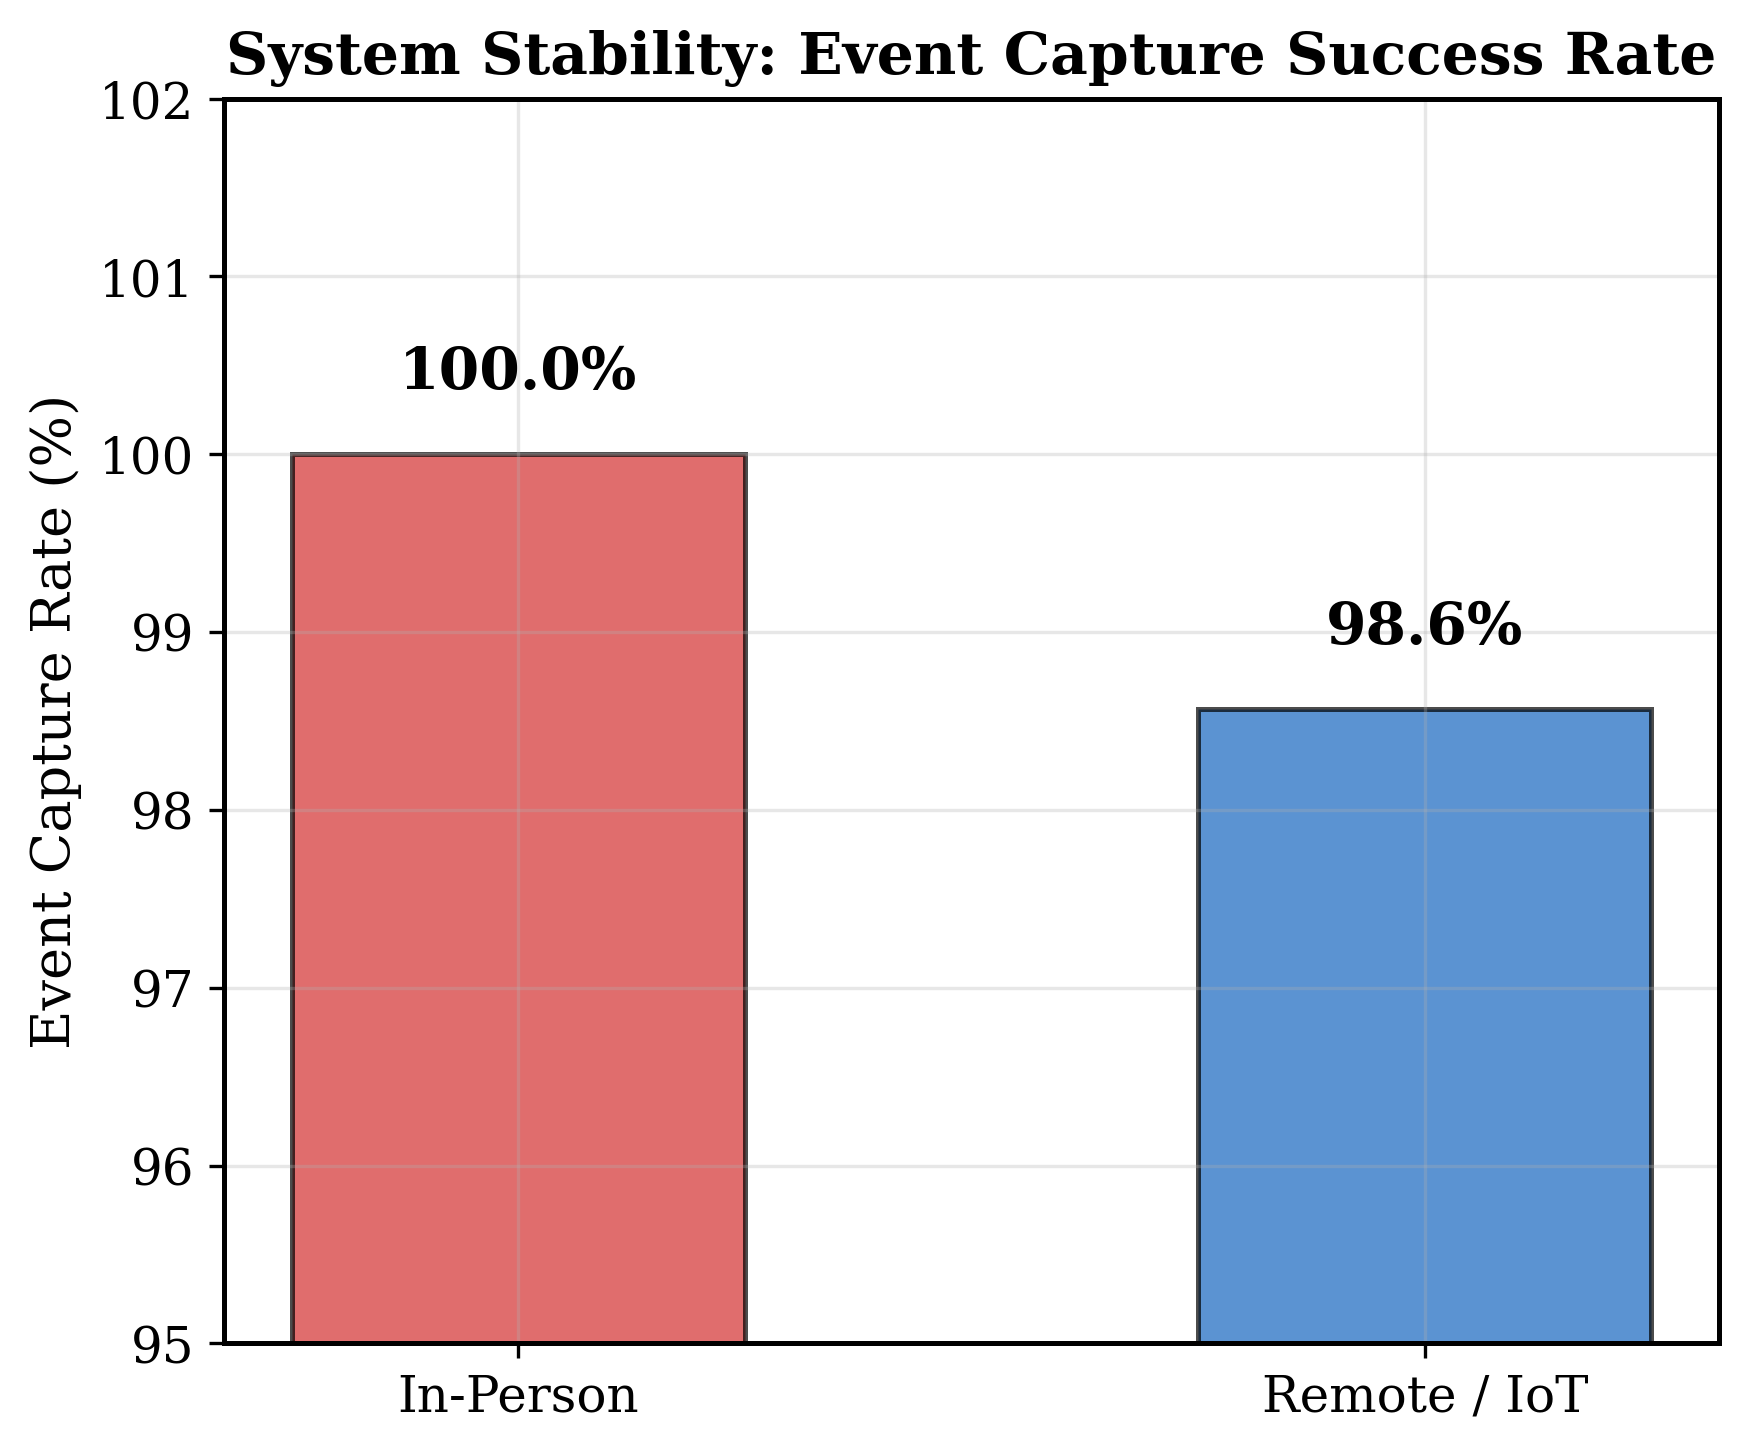
\includegraphics[width=0.70\textwidth]{../figures/stability_success_rate.png}
\end{figure}

\textbf{S\'intesis de resultados.} En conjunto, los resultados muestran una alta concordancia entre ambas modalidades: diferencias de medias inferiores a 0{,}03~s, variaciones de desviaci\'on est\'andar menores a 0{,}02~s, ausencia de sesgo sistem\'atico confirmada por Bland--Altman y aceleraciones experimentales id\'enticas en ambas modalidades. Estos hallazgos constituyen evidencia cuantitativa de que el sistema IoT no introduce errores sistem\'aticos en las mediciones cinem\'aticas y reproduce con alta fidelidad el comportamiento f\'isico del experimento de MRUA.

\subsection{Discusi\'on}

El aporte cient\'ifico central de este trabajo radica en establecer un protocolo de validaci\'on cuantitativa para sistemas IoT aplicados a experimentos f\'isicos cl\'asicos, contribuyendo a cerrar la brecha identificada en la literatura entre implementaci\'on tecnol\'ogica y rigor cient\'ifico. A diferencia de estudios previos centrados en la demostraci\'on funcional de laboratorios remotos, este trabajo proporciona evidencia estad\'istica formal ---mediante prueba~t para muestras independientes, an\'alisis de Bland--Altman y tasa de captura de eventos--- de que un sistema IoT de bajo costo puede reproducir con precisi\'on comparable las mediciones cinem\'aticas de un montaje presencial. Este resultado tiene implicaciones directas para el dise\~no de pol\'iticas de modernizaci\'on de infraestructura educativa en contextos de recursos limitados.

Los resultados obtenidos demuestran que el sistema de \textit{retrofitting} IoT es capaz de capturar la din\'amica del MRUA con fidelidad experimental comparable al montaje presencial tradicional, superando as\'i la limitaci\'on m\'as frecuente en la literatura: la ausencia de validaci\'on cuantitativa rigurosa. A diferencia de estudios previos que enfatizan la implementaci\'on funcional de laboratorios remotos~\parencite{r2,r5}, este trabajo aporta evidencia cuantitativa directa de la equivalencia experimental, estableciendo un precedente metodol\'ogico aplicable a otros experimentos de f\'isica cl\'asica.

La efectividad del procesamiento Edge computing en el m\'odulo ESP32 queda demostrada por la pr\'actica nulidad del sesgo entre modalidades: la latencia de red, aunque presente en la transmisi\'on MQTT, no afect\'o la calidad de las marcas temporales registradas. Este hallazgo es coherente con los principios formulados por~\textcite{r7} respecto a la reducci\'on de latencia efectiva mediante Edge computing en entornos educativos IoT.

El coeficiente de correlaci\'on de Pearson calculado entre ambas series result\'o estad\'isticamente no significativo ($r \approx 0$), resultado te\'oricamente esperado para series independientes que comparten la misma fuente de variabilidad f\'isica estoc\'astica. Como se\~nalan~\textcite{giavarina2015}, este valor no refleja una limitaci\'on instrumental sino la naturaleza no pareada del dise\~no experimental, que queda adecuadamente validado mediante las pruebas~t y Bland--Altman. El an\'alisis Bland--Altman completa la evaluaci\'on al confirmar que no existen sesgos sistem\'aticos, lo que resulta suficiente para validar la equivalencia experimental a efectos did\'acticos~\parencite{bland1986}.

Desde una perspectiva comparativa, el sistema propuesto contrasta favorablemente tanto con soluciones comerciales como con trabajos acad\'emicos recientes. Las soluciones comerciales para laboratorios remotos suelen implicar costos superiores a USD~500 por estaci\'on y sistemas propietarios con limitada adaptabilidad~\parencite{r4}. La propuesta desarrollada, con un costo total inferior a USD~150, utiliza hardware de consumo masivo y c\'odigo de fuente abierta, manteniendo niveles de precisi\'on estad\'isticamente equivalentes. Respecto a arquitecturas similares basadas en ESP32 y Raspberry Pi~\parencite{r10}, la diferencia central de este trabajo radica en la validaci\'on cuantitativa de la equivalencia cinem\'atica entre modalidades, ausente en los trabajos de referencia.

En s\'intesis, la combinaci\'on de prueba~t para muestras independientes, prueba de Levene y an\'alisis Bland--Altman constituye un protocolo de validaci\'on multidimensional que puede adoptarse como est\'andar para futuros desarrollos de sistemas remotos en f\'isica experimental, superando las limitaciones de m\'etricas \'unicas como el coeficiente de correlaci\'on.

\subsection{Limitaciones}

El estudio presenta cuatro limitaciones que deben considerarse al interpretar los resultados. Primera, la validaci\'on se limita a un \'unico experimento (MRUA) en un entorno controlado; la extensi\'on a otros experimentos de din\'amica y energ\'ia es parte del trabajo futuro. Segunda, el sistema depende de la disponibilidad continua del servidor MQTT y de la calidad de la red WiFi, factores que pueden afectar la tasa de captura en entornos con conectividad inestable. Tercera, aunque el tama\~no muestral ($n=35$ por modalidad) fue determinado mediante an\'alisis de potencia \textit{a priori}, estudios con muestras m\'as amplias y dise\~nos experimentales pareados permitir\'ian an\'alisis de concordancia m\'as precisos. Cuarta, \textbf{el estudio no incluy\'o mediciones expl\'icitas de latencia en la cadena de comunicaci\'on} (ESP32~$\to$ MQTT~$\to$ backend~$\to$ interfaz web), lo que limita la caracterizaci\'on completa del comportamiento temporal del sistema bajo distintas condiciones de red; esta medici\'on se incluir\'a en versiones futuras del prototipo.

%========================================================
\section{Conclusiones}

Este trabajo present\'o el dise\~no, implementaci\'on y validaci\'on cuantitativa de un sistema de \textit{retrofitting} IoT para el estudio experimental del MRUA en un entorno h\'ibrido de aprendizaje. Los resultados demuestran que el sistema propuesto reproduce las mediciones cinem\'aticas del montaje presencial de referencia con alta fidelidad experimental: las diferencias de medias son inferiores a 0{,}03~s en todos los puntos de medici\'on, las desviaciones est\'andar difieren en menos de 0{,}02~s, y las aceleraciones experimentales medias son pr\'acticamente id\'enticas en ambas modalidades ($\mu \approx 0{,}95$~m/s$^2$). El an\'alisis de Bland--Altman confirm\'o la ausencia de sesgo sistem\'atico entre modalidades ($|\overline{d}| < 0{,}002$~s), y la tasa de captura exitosa de eventos alcanz\'o el 98{,}5\% en modalidad remota.

La contribuci\'on central de este trabajo es la validaci\'on cuantitativa de la equivalencia experimental entre modalidades remota y presencial, estableciendo que un sistema IoT de bajo costo (<~USD~150) basado en Edge computing con ESP32 puede replicar con precisi\'on comparable las mediciones de un montaje presencial de cinem\'atica. Este resultado tiene implicaciones directas para la modernizaci\'on de infraestructuras educativas en contextos de recursos limitados, demostrando que el \textit{retrofitting} IoT permite transformar equipamiento cl\'asico en activos digitales conectados sin requerir su sustituci\'on.

El potencial del \textit{retrofitting} IoT para modernizar laboratorios educativos h\'ibridos queda as\'i demostrado en este estudio, que aporta un protocolo de validaci\'on replicable ---combinando prueba~t para muestras independientes, prueba de Levene y an\'alisis Bland--Altman--- aplicable a otros experimentos de f\'isica cl\'asica. La arquitectura de tres capas con c\'odigo de fuente abierta publicado en GitHub~\parencite{r15} es directamente replicable en laboratorios con recursos similares.

Las l\'ineas de investigaci\'on futura incluyen: (1)~extensi\'on del sistema a experimentos de din\'amica, energ\'ia y ondas; (2)~evaluaci\'on del aprendizaje con grupos reales de estudiantes; (3)~integraci\'on con sistemas LMS (Moodle, Canvas); (4)~incorporaci\'on de sensores de mayor resoluci\'on temporal; (5)~medici\'on expl\'icita de latencia en la cadena de comunicaci\'on; y (6)~implementaci\'on de QoS nivel~1 en MQTT para redes inestables.

%========================================================

\section{Reconocimientos y declaraciones}

\subsection{Agradecimientos}
El desarrollo y evaluaci\'on del prototipo se realizaron con la autorizaci\'on expl\'icita de la Pontificia Universidad Cat\'olica del Ecuador, sede Esmeraldas, tanto para el uso del laboratorio de f\'isica como para la menci\'on de la instituci\'on en el manuscrito.

%========================================================
\subsection{Contribuciones de autor\'ia}
Conceptualizaci\'on, W.S.S.M. y M.R.N.T.; metodolog\'ia, W.S.S.M. y M.R.N.T.; software, W.S.S.M.; validaci\'on, W.S.S.M. y M.R.N.T.; an\'alisis formal, W.S.S.M.; investigaci\'on, W.S.S.M.; recursos, M.R.N.T.; curaci\'on de datos, W.S.S.M.; redacci\'on del borrador original, W.S.S.M.; revisi\'on y edici\'on, W.S.S.M. y M.R.N.T.; visualizaci\'on, W.S.S.M.; supervisi\'on, M.R.N.T.; administraci\'on del proyecto, M.R.N.T. Todos los autores han le\'ido y aprobado la versi\'on final del manuscrito.

\subsection{Declaraci\'on sobre el uso de inteligencia artificial}
Los autores declaran que, durante la elaboraci\'on del art\'iculo, se utiliz\'o ChatGPT de OpenAI como apoyo para la elaboraci\'on de diagramas y la revisi\'on de redacci\'on, y Gemini de Google para la generaci\'on de im\'agenes. Los autores verificaron y asumieron la responsabilidad del contenido final.

\subsection{Conflictos de inter\'es}
Los autores declaran que no existen conflictos de inter\'es.

\printbibliography[title={Referencias}]
\end{document}
